% 14.06.2019, markus endres

% delete „english“ if you are writing a thesis in German.
\documentclass[11pt,fleqn,a4paper,headsepline, numbers=noenddot,bibliography=totoc,oneside, version=first,listof=totoc,ngerman,english]{scrreprt}

\usepackage{scrhack}
\usepackage{finalthesis}
\usepackage{fancyheadings}

\usepackage{pdfsync}
%\usepackage{ngerman,english}
\usepackage[ngerman,english]{babel}
\usepackage[backend=biber,sorting=none,style=numeric,language=english]{biblatex}
\usepackage[utf8]{inputenc} 
\usepackage{epsfig}

\usepackage[all]{xy}
\usepackage{a4wide}
\usepackage{longtable,multicol}
\usepackage{eurosym}
\usepackage{alltt}
\usepackage[small, bf]{caption}
\usepackage{helvet}
\usepackage[hidelinks]{hyperref}
\usepackage{setspace}
\usepackage[active]{srcltx}
\usepackage{cancel}
\usepackage{eepic}
\usepackage{epic}
\usepackage{enumerate}
\usepackage{color}
\usepackage{xcolor}
\usepackage{colortbl}
\usepackage{bigstrut}
\usepackage{amssymb}
\usepackage{amsmath}
\usepackage{amsthm} 
\usepackage{algorithm}
\usepackage{algpseudocode}
\usepackage[normalem]{ulem}
\usepackage[nomain, abbreviations]{glossaries-extra}

\usepackage{lscape}

\usepackage{listings}
\lstset{language=}
\lstset{basicstyle=\ttfamily}
\lstdefinelanguage{PSQL}[]{SQL}{
   morekeywords={PREFERRING}
   sensitive=true,% DJ
   morecomment=[l]--,%
   morecomment=[s]{/*}{*/},%
   morestring=[d]',%
   morestring=[d]"%
}[keywords,comments,strings]%

% better bibliography (biblatex style)
% use biber to compile
\usepackage[autostyle,english=american,german=quotes]{csquotes}
\usepackage{amsmath}  % for \hookrightarrow
\usepackage{xcolor}   % for \textcolor
\usepackage{multirow}
\usepackage{rotating}
\usepackage{array}
\usepackage{enumitem} % http://ctan.org/pkg/enumitem
\usepackage{vcell}
\usepackage{graphicx}

\addbibresource{literature.bib}


\newcommand{\pareto}{\otimes}
\newcommand{\prio}{~\&~}
\newcommand{\indiff}[3]{#1\ \|_{#2}\ #3}
\newcommand{\antichain}[1]{#1^\leftrightarrow}

%\newtheorem{definition}{Definition}
\newtheorem{theorem}{Theorem}
\newtheorem{corollary}{Corollary}
\newtheorem*{theoremproof}{Proof}
\newtheorem{lemma}{Lemma}
\newtheorem*{lemmaproof}{Proof}
\newtheorem{example}{Example}
\newtheorem{def_internal}{Definition}
\newenvironment{definition}[1]{
  \begin{def_internal}{\textbf{#1}\\}
}{ 
  \hfill $\Box$
  \end{def_internal}
}

\renewcommand{\algorithmiccomment}[1]{$\rhd$ #1 \hfill}
\renewcommand{\labelenumi}{\alph{enumi})}
\renewcommand{\algorithmiccomment}[1]{//#1 }

\renewcommand{\sectfont}{\rmfamily\bfseries}
\renewcommand{\topmargin}{0mm}
\renewcommand{\textheight}{222mm}
%\renewcommand{\textwidth}{152mm}
%\renewcommand{\evensidemargin}{-2mm}
%\renewcommand{\oddsidemargin}{29mm}
%\setlength{\oddsidemargin}{1.8cm}

\setcounter{topnumber}{3}
%\renewcommand{\baselinestretch}{1.09}

\setlength{\mathindent}{0.5cm}
\setlength{\parindent}{0cm}
\setlength{\parskip}{1.2ex plus0.5ex minus0.2ex}
\setcounter{secnumdepth}{5}

\setcounter{tocdepth}{5}
\renewcommand{\textfraction}{0.0}

%
% Kopfzeile
%
\pagestyle{fancyplain}
\renewcommand{\chaptermark}[1]{\markboth{#1}{}}
\renewcommand{\sectionmark}[1]{\markright{\thesection\ #1}}
\lhead[\fancyplain{}{\bfseries\thepage}]
 {\fancyplain{}{\bfseries\rightmark}}
\rhead[\fancyplain{}{\bfseries\leftmark}]
 {\fancyplain{}{\bfseries\thepage}}
\cfoot{\fancyplain{\bfseries\thepage}{}}
%Background
\newabbreviation{csr}{CSR}{Certificate Signing Request}
\newabbreviation{mac}{MAC}{Message Authentication Code}
\newabbreviation{ofmc}{OFMC}{Open-source Fixed-point Model Checker}
\newabbreviation{smp}{SMP}{Socialist Millionaires' Protocol}

%%%%%%%%%%%%% use cases %%%%%%%%%%%

\newabbreviation{pki}{PKI}{Public Key Infrastructure}
%ABC use case
\newabbreviation{abc}{ABC}{Automated Border Control}
\newabbreviation{das}{DAS}{Document Authentication System}
\newabbreviation{bvs}{BVS}{Biometric Verification System}
\newabbreviation{csi}{CSI}{Central Systems Interface}
\newabbreviation{bgms}{BGMS}{Border Guard Maintenance System}
\newabbreviation{vms}{VMS}{Visa Management System}
\newabbreviation{rtp}{RTP}{Registered Traveler Program}
\newabbreviation{eems}{EEMS}{Entry-Exit Management System}

%IoT use case
\newabbreviation{tcp}{TCP}{Transmission Control Protocol}
\newabbreviation{udp}{UDP}{User Datagram Protocol}
\newabbreviation{iot}{IoT}{Internet of Things}
\newabbreviation{tls}{TLS}{Transport Layer Security}
\newabbreviation{dtls}{DTLS}{Datagram Transport Layer Security}
\newabbreviation{ietf}{IETF}{Internet Engineering Task Force}
\newabbreviation{coap}{CoAP}{Constrained Application Protocol}
\newabbreviation{rest}{REST}{Representational state transfer}

%Bootstrapping
\newabbreviation{idevid}{IDevID}{Initial Device Identifier}
\newabbreviation{ldevid}{LDevID}{Locally Significant Device Identifier}
\newabbreviation{p2p}{P2P}{Peer-to-Peer}
\newabbreviation{brski}{BRSKI}{Bootstrapping Remote Secure Key Infrastructure}
\newabbreviation{sztp}{SZTP}{Secure Zero Touch Provisioning}
\newabbreviation{oob}{OOB}{Out-Of-Band}
\newabbreviation{eap-tls}{EAP-TLS}{Extensible Authentication Protocol TLS}
\newabbreviation{gba}{GBA}{Generic Bootstrapping Architecture}
\newabbreviation{est}{EST}{Enrollment over Secure Transport}
\newabbreviation{ca}{CA}{Certification Authority}
\newabbreviation{masa}{MASA}{Manufacturer Authorized Signing Authority}
\newabbreviation{ra}{RA}{Registration Authority}
\newabbreviation{ee}{EE}{End Entity}
\newabbreviation{dos}{DoS}{Denial of Service}
\newabbreviation{scram}{SCRAM}{Salted Challenge Response Authentication Mechanism}
\newabbreviation{tofu}{TOFU}{Trust on first use}
\newabbreviation{nea}{NEA}{Network Endpoint Assessment}
\newabbreviation{cmp}{CMP}{Certificate Managment Protocol}
\newabbreviation{nms}{NMS}{Network Managment System}
\newabbreviation{rstcnf}{RESTCONF}{Representational State Transfer Configuration}

%post compromise security
\newabbreviation{otr}{OTR}{Off-the-Record}
\newabbreviation{rke}{RKE}{ratcheted key exchange}
\newabbreviation{nist}{NIST}{National Institute of Standards and Technology}
\newabbreviation{ec}{EC}{Elliptic Curve}
\newabbreviation{ecdh}{ECDH}{Elliptic Curve Diffie-Hellmann}
\newabbreviation{sidh}{SIDH}{Supersingular isogeny Diffie-Hellman}
\newabbreviation{kem}{KEM}{Key Encapsulation Mechanism}
\newabbreviation{ake}{AKE}{authenticated key exchange}

%x3dh
\newabbreviation{x3dh}{X3DH}{Extended Triple Diffie-Hellmann}
\newabbreviation{otp}{OTP}{One Time Pre-key}
\newabbreviation{ik}{IK}{Identity Key}

%DR
\newabbreviation{0rtt}{0-RTT}{Zero Round Trip Time}
\newabbreviation{kdf}{KDF}{Key Derivation Function}
\newabbreviation{dh}{DH}{Diffie-Hellmann}
\newabbreviation{rk}{RK}{Root Key}
\newabbreviation{ck}{CK}{Chain Key}
\newabbreviation{hk}{HK}{Header Key}
\newabbreviation{nhk}{NHK}{Next Header Key}

\makeglossaries
\usepackage{chngcntr}
\counterwithout{footnote}{chapter}

\begin{document}


%%%%%%%%%%%%%%%%%%%%%%%%%%%%%%%%%
% Modify this
%%%%%%%%%%%%%%%%%%%%%%%%%%%%%%%%%
% Bachelor or Master thesis}
\ftgrad{Master Thesis}
% title
\fttitle{Secure Bootstrapping and Post-Compromise Security in IoT}
% Author
\ftauthor{Hossam Hamed}
% 1. examiner
\ftgutachter{Prof. Dr. Joachim Posegga}
% 2. examiner
% Delete this line if you write a Bachelor thesis
\ftzweitgutachter{Prof. Dr. Jorge Cu\'{e}llar}
% supervisor
\ftbetreuer{Prof. Dr. Jorge Cuellar}
% date of submission
\ftdate{\today}

%%%%%%%%%%%%%%%%%%%%%%%%%%%%%%%%%

\makefttitle


\pagenumbering{roman}

\tableofcontents
\newpage

% Abstract
% !TeX spellcheck = en_US
% !TeX encoding = UTF-8
\chapter*{Abstract}
\gls{iot} is being hailed as one of the primary catalysts of the next digital revolution. The technology enables connecting ubiquitous objects to the internet. 
Security is an essential aspect of the different phases of the lifecycle of an IoT device.
In particular, our thesis is primarily focused on discussing the security of the bootstrapping phase and management of cryptographic keys during the operational phase to ensure desired security features for the utilized keys.
The first goal of this thesis is to examine the significance of secure zero-touch bootstrapping of IoT devices. We analyze and present a comparison between two bootstrapping protocols: \gls{brski} and \gls{sztp}. 
Secondly, we aim to discuss the future secrecy of cryptographic keys in IoT through analyzing the \gls{x3dh} protocol and the double ratchet algorithm. In addition to use \gls{ofmc} to formally verify a model of a \gls{x3dh} protocol variant. Moreover, provide an implementation for the future secrecy related protocols.
Thirdly, we discuss the applicability of the mentioned protocols in IoT-related use cases.
Lastly, we aimed at conducting a comparative study between certificate enrollment protocols.
Although the thesis does not finally conclude the discussion of IoT security, we have shown than that the mentioned bootstrapping protocols
Regarding X3DH protocol and the double ratchet algorithm, they are viable solutions and applicable to IoT and provide and enhance security in the proposed scenarios.

\newpage

% Acknowledgements (optional)
\chapter*{Acknowledgments}

First and foremost, I sincerely thank Prof. Dr. Jorge Cu\'{e}llar for his continuous guidance, endless support, and patience. I have benefited immensely from his wealth of knowledge throughout this master's degree. It has been my pleasure to be his student and work under his supervision. I would also like to express my appreciation to the University of Passau, specifically the chair of IT-Security.

I am incredibly grateful for my family's unconditional, unequivocal, and loving support that they give in all possible forms. Without their encouragement and prayers in each and every step of this journey, it would not have been possible. Nonetheless, I want to express my gratitude to my dear friend Franz Stimmer for his continuous support and encouragement since the day when coming to Germany was just an idea.

Last but not least, I would like to show my appreciation for the incredible friends I have made over the past years through this journey. They have made hard days bearable and good days even better.


\newpage




%\addcontentsline{toc}{chapter}{Abbildungen}
\listoffigures
%\addcontentsline{toc}{chapter}{Tabellen}
\listoftables
\printunsrtglossaries

%%%%%%%%%%%%%%%%%%%%%%%%%%%%%%%%%%%%%%%%%%%%%
\chapter{Introduction}
\label{ch:introduction}

\gls{iot} is a relatively new concept that already has applications in many domains, creating new ways of interactions between humans and small devices, referred to as smart devices. Applications like Smart Airports, Transportation, Home Automation, and many more are being revolutionized by this technology \cite{marksteiner2017overview}.
\gls{iot} is the deployment of network-connected constrained devices that interact with the physical environment by employing sensors to collect data, managing other systems, controlling actuators, as well as communicating with one another. \gls{iot} devices are classified into several classes depending on their degree of computing resources and power usage. Depending on their degree, they may be assumed to not be able to process sophisticated or even conventional cryptographic operations. In many use cases, the \gls{iot} devices handle critical and private data. This imposes the requirement for data integrity and authenticity guarantees, and -because of privacy- in many cases also confidentiality.
\par
IoT device life cycle and nature of IoT communication 

%\gls{tls} \cite{rfc5246}, which relies on \gls{tcp}, has been criticized as inappropriate for constrained \gls{iot} devices \cite{shang2016challenges}. Among the reasons are, the infeasibility of \gls{iot} devices to maintain long-lived connections due to energy constraints, high header overhead, and the low-latency requirement that is opposed by the delay due to \gls{tcp} handshake, especially in a lossy network.
%Alternatively, \gls{dtls} \cite{dtls} provides security for communication channels relying on \gls{udp}. In contrast to \gls{tcp}, \gls{udp} is more suitable for \gls{iot}. It is an unreliable protocol as it does not care about message delivery , resulting in a lower header overhead. In addition, it introduces less traffic to the network.
%\par
%The \gls{ietf} introduced \gls{coap} \cite{rfc7252} that is intended to be a generic application protocol for constrained environments. Similar to the ubiquitous HTTP \cite{http}, \gls{coap} realizes a subset of the \gls{rest} architecture. Therefore, it easily translates to HTTP. Moreover, \gls{coap} leverages \gls{udp} as its transport layer protocol which is secured by \gls{dtls}. Hence, \gls{coap} is one of well-suited protocols for \gls{iot}.

\section{Research Questions and Contributions}\label{sec:reserach_questions}
research questions: motivate the desire for zero-touch bootstrapping and future secrecy.
\par
The contributions of the thesis are the following:
\begin{itemize}
	\item We conduct a comparative study between two secure bootstrapping protocols, \gls{brski} and \gls{sztp}.
	\item We give an overview over the \gls{x3dh} protocol and the double ratchet algorithm. In addition to present a formal verification of the \gls{x3dh} using \gls{ofmc}. Moreover, we reflect on stand of those protocols in the post-quantum setting.
	\item We provide a demo implementation for \gls{x3dh} and the double ratchet algorithm using Python.
	\item Although not strictly relevant, we present a comparison table between a set of certificate enrollment protocols in appendix \ref{appendix-enrollment}.
\end{itemize}

\section{Structure of the Thesis}\label{sec:structure_of_the_thesis}

The structure of this thesis is as follows: In chapter \ref{ch:background}, we reflect on principles relevant to the understanding of the work presented in further chapters. In addition to other works related to our thesis. 
Next we propose real-world use cases in chapter \ref{ch:usecases} where the protocols to be proposed can be applied.
In chapter \ref{ch:secureBootstrapping}, we give an overview of the two promising automated bootstrapping protocols: \gls{brski} and \gls{sztp}. Moreover, we present a comparative study between them.
Chapter \ref{ch:postcomp} discusses post-compromise security, and how it is achievable in an asynchronous environment through the use of \gls{x3dh} and double ratcheting. In addition, we discuss the formal verification of the protocols and their stand in the world of quantum computing.
In chapter \ref{ch:implementation} we present our demo implementation of the protocols discussed in chapter \ref{ch:secureBootstrapping}. 
Furthermore, chapter \ref{ch:discussion} discusses our findings and reflects the represented protocols on the use cases.
Finally, chapter \ref{ch:conclusion} concludes our work and introduces suggestions for future work. 
\chapter{Background}
\label{ch:background}

This chapters gives an overview over concepts important for the protocols and algorithms discussed in further chapters.
\section{Preliminaries}

\subsection{Certificate}

\subsection{Encryption}
	\subsubsection{Symmetric Encryption}
	\subsubsection{Asymmetric Encryption}
	
\subsection{Bootstrapping}

\subsection{Voucher Artifact}

\subsection{Certificate Enrollment}

\subsection{Protocol Formal Modeling}

\subsection{\acrfull*{kdf}} \label{backgroung:kdf}

\subsection{Threat Models}

\subsection{Secure Messaging}
	
	\subsubsection{properties}
	%	
	%	\item Forward Secrecy:
	%	
	%	\item Future Secrecy:
	%		- abstract ... explained in post-comp chapter
	%	\item immediate decryption:
	%		the fact that messages might arrive out of order or be lost entirely. Additionally, parties can be offline for extended periods of time and send and receive messages asynchronously. Given these inherent constraints, immediate decryption is a very attractive feature. Informally, it ensures that when a legitimate message is (eventually) delivered to the recipient, the recipient can not only immediately decrypt the message but is also able to place it in the correct spot in relation to the other messages already received. Furthermore, immediate decryption also ensures an even 	more critical liveness property, termed message-loss resilience (MLR) in this work: if a message is permanently lost by the network, parties should still be able to communicate
	
	
\section{Related Work}
	\subsection{OTR}
	\subsection{SoK}
	\subsection{Key Continuity Management}
	\subsection{On post-compromise security}
	study post-compromise security 	in (classic) key exchange. Here, security shall be achieved even for sessions established after a full compromise of user secrets. This necessarily requires mixing user state information with key material that is newly established via asymmetric techniques, and is thus related to RKE.
	\subsection{Tesla}
\chapter{Use Cases}
\label{ch:usecases}

\section{Automated Border Control (ABC)}
International passenger traffic has been monitored to continuously increase over the years. Since air transport is one of the most convenient form of long distance transport among passengers, the above claim is indicated by the Airports Council International's Passenger Traffic Summary \footfullcite{aci_world_2019}. Despite the current shock due to the Covid-19 pandemic to the air transport industry, the aviation industry has shown resilience over the past decades and is predicted to recover and further grow by $ 4\% $ over the course of the next 20 years \footfullcite{Boeing2020} international border crossing points are forecasted to face more traffic than they already are. Implying the requirement for a solution to the Border control process to mitigate longer queues and waiting times, or the need to hire and train more personnel to conduct the task.
\par
Bio-metric passports are widely issued by more than 150 countries and regions, as of 2020 \footfullcite{ReadID2020}. Such passports contain a contactless smart chip that stores the passport holder's bio-metric information to authenticate his identity at passport control stations. The chips may contain one or more of the following bio-metric data: Iris, Fingerprint, and/or Facial features. In recent years, \gls{abc} systems, or E-Gates, started rolling out in airports leveraging the wide deployment of bio-metric passports. They intend to automate the process and improve the management and control of travel flows, serving passengers in a shorter time and reduce queues at airports. Resulting in benefits to the Aircraft operators, Airports, passengers, and Governments \cite{Angiolelli-meyer2015}.
\par
% types of E-gates
%- modules and services in the E-gate
Labati et al. \cite{labati2016biometric} represented two types of communication performed at an E-Gate: communication between systems interconnected within the E-Gate, and communication with External systems. Internally, an E-Gate is composed of 4 subsystems: \gls{das}, \gls{bvs}, \gls{csi}, and \gls{bgms}. Externally, the E-gate is part of a larger border control infrastructure. It communicates with external systems to query for additional information to verify the traveler's eligibility to be granted access to cross the border. An E-Gate can query the databases of the following external systems: \gls{vms}, \gls{rtp}, and \gls{eems}. Figure \ref{E-Gate-Architecture} from \cite{labati2016biometric} presents an illustrative overview of the E-Gate logical architecture. Essentially, the data transfer between the above systems, internally and externally, must be secure as it includes personal data, bio-metrics, and decision making information that affect a state's national security.
\begin{figure}[H]
	\centering
	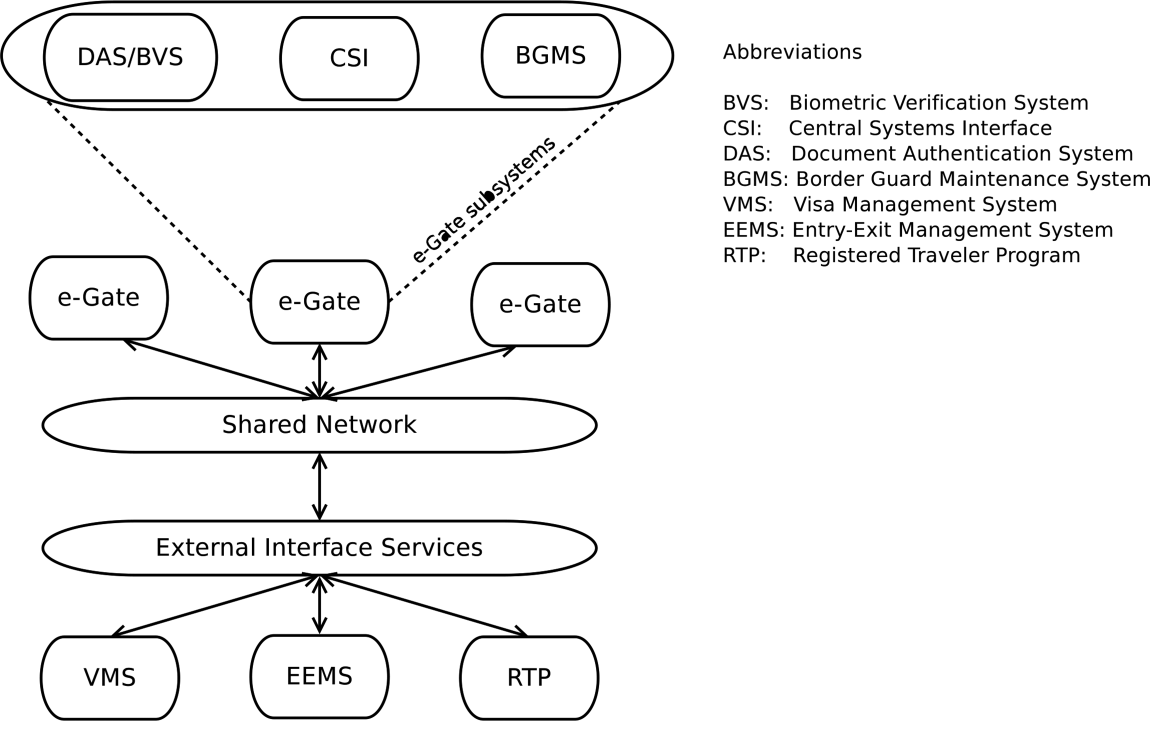
\includegraphics[scale=0.35]{Images/E-Gate-Architecture.png}
	\caption{ABC Logical Architecture overview \cite{labati2016biometric}}
	\label{E-Gate-Architecture}
\end{figure}

\par
The workflow of the ABC systems is similar to the one depicted in Figure \ref{workflow}. At first, a citizen starts by scanning his passport data page through the gate's scanner. The scanner communicates the image to the Border control system (BCS) which in turn runs its optical data recognition software to extract the data from the scanned data page and verify the document security features. Next, the E-Gate proceeds by reading the embedded electronic chip in the passport. Due to the sensitivity of the bio-metric data, they are not transferred. However, the non-sensitive data stored on the chip, which is equivalent to the data already scanned, is sent to the BCS to cross-check the passport data page. The citizen's facial features and bio-metrics are scanned by the E-Gate to authenticate the citizen against the chip's data. Finally, If the BCS verifies the passport, the E-Gate verifies the bio-metric features, and no match was found in the BCS's watchlists, then the citizen is allowed to pass the border checkpoint.

\begin{figure}[H]
	\centering
	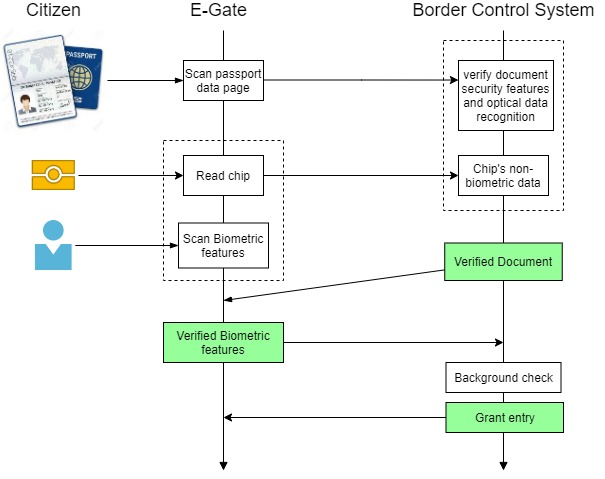
\includegraphics[scale=0.3]{Images/ABC.jpeg}
	\caption{Workflow of ABC.}
	\label{workflow}
\end{figure}
%attacks on E-Gates (facial recognition)

\section{Internet of Things (IoT)}
Industry 4.0, or the Fourth Industrial Revolution, refers to the 21st century's swift advances in technology, industry, and societal patterns and processes. Industry 4.0 is the concept of using automation and data exchange in manufacturing. Nine pillars of technologies make up Industry 4.0; among them are the Industrial Internet of Things (IIoT) and Cybersecurity. These technologies are used to create a ``smart factory" where sensors, machines, systems, and humans communicate with each other in order to control and monitor progress throughout the manufacturing process digitally.
\par
IIoT is a method of digitally transforming manufacturing. It relies on a network of sensors to gather essential production data, then leverages linked systems and infrastructure to transform that data into beneficial insights about the effectiveness of the industrial processes. Likewise, Cybersecurity is a vital foundation of IIoT. Industry 4.0 and IoT demand linking together independent devices and systems from possibly different vendors while one device’s action is based on the output of another device. This translates to a substantial increase in connectivity directly related to an increase in the risk of potential cyber-attacks.
IoT devices in the industrial realm interact and generate an enormous amount of data in different aspects. For example, employees' wearable devices to share information, alerts, and monitor their health status, smart production line machines, inventory environment sensors, and connected transportation vehicles.	The data within IIoT environments is critically sensitive as it directly affects employees', customers', and manufacturers' privacy, manufacturer's operations and market competitiveness, and functional safety.
A relevant incident that highlights the importance of cybersecurity in the industrial field is the infamous Stuxnet attack\footnote{https://www.wired.com/2014/11/countdown-to-zero-day-stuxnet/}. It is an attack against an Iranian uranium enrichment plant where the attack technically manipulated the enrichment centrifuges causing them to fail. Therefore, it is crucial for industrial information systems and manufacturing processes against cyber threats as a security breach can affect multiple areas, from supply chain to operations.


\section{V2V}
- define v2v\\
- architectural overview of v2v\\
- use case messages\\
- secure communication (Tesal, etc...)\\



\chapter{Secure Bootstrapping}
\label{ch:secureBootstrapping}
The term ``Bootstrapping" is used in a spectrum of contexts including Computing, Law, Finance\footfullcite{bs-wiki}. It is inspired from the late idiom ``to pull oneself up by one's bootstraps" which means to succeed or elevate yourself without any outside help. In the context of Networking, bootstrapping is an initial procedure between an unconfigured devices which intend to communicate with a network for the first time. Its goal is to provide the device with the required information that enables it to establish subsequent secure communication channels with the desired network. Such information can be certificates, configurations, and metadata.
\par
Integrity and confidentiality of information flow between the two ends of the communication are are what defines end to end secure channels. Authentication, whether unilateral or mutual, is another fundamental aspect to achieve channel security. Existing protocols, such as \gls{tls}, can achieve End-to-end security between parties. However, analogous protocols rely digital certificates and credentials which are managed by local or third party \gls{pki}. Therefore to ensure correct and secure execution of protocols certificates must be securely provisioned to their corresponding identities. Typically at the manufacturing phase, the manufacturer usually installs globally unique manufacturer provided identifiers known as the \gls{idevid} \cite{5367679}. Its main use is for identity verification purposes and it should not be used to enforce data integrity nor confidentiality. Upon successful completion of the bootstrapping process, the device should posses identifiers that allows for subsequent establishment of secure channels with the network domain. An identifier in this set of identifiers is known as \gls{ldevid} \cite{5367679}.
\par
Bootstrapping approaches differ in the degree of manual user involvement and the amount of information on the device which must be pre-configured by the manufacturer. The survey by Sethi et al. \cite{irtf-t2trg-secure-bootstrapping-00} provides a classification for Bootstrapping mechanisms into general categories: Managed methods, \gls{p2p} and Ad-hoc methods, Opportunistic methods, and Hybrid methods.
\begin{itemize}
	\item \textit{Managed methods}: These bootstrapping approaches count on pre-established credentials and trust anchors for authentication and security. The required initial information and cryptographic material can be acquired either at manufacture time in the factory, or through \gls{oob} means, e.g. using a smart card or a USB. Examples of this method are \gls{eap-tls} \cite{eap-tls} and \gls{gba} \cite{gba}.
	
	\item \textit{\gls{p2p} methods}: Contrary to managed methods, these bootstrapping methods do not rely on any pre-established cryptographic material or information. Instead, the bootstrapping protocol results in credentials being established for subsequent secure communication. Typically, resulting credentials are authenticated using an \gls{oob} channel. This category of methods may be utilized if the manufacturer is incapable or untrustworthy to generate the desired credential.
	
	\item \textit{Opportunistic methods}: Unlike previous methods where the authenticity of the initially presented identity is verified, approaches which fall under this category rely on verification of the continuity of the initial identity provided. Bergmann et al. \cite{simplekeys} have developed a secure bootstrapping mechanism that is an example of this category. 
	
	\item \textit{Hybrid methods}: A wide range of deployed approaches use components from both managed and \gls{p2p} methods. Such approaches are categorized as hybrid methods.	
\end{itemize} 

This chapter discusses two voucher-based bootstrapping protocols that aim at being zero touch protocols by eliminating the user interference. These protocols are \gls{brski} \cite{brski} and \gls{sztp} \cite{sztp}. Both protocols fall under the managed methods category.

%brski section
\section{\acrfull*{brski}}
%intro
\gls{brski} is a product of the ANIMA working group of the \gls{ietf}. It is an automated bootstrapping protocol that enables an unconfigured device to discover and securely join an unfamiliar network domain it is installed in. \gls{brski} results in the device acquiring an X.509 root certificate to authenticate the network domains' elements and establish consecutive secure channels. Moreover, the device can use the obtained certificate to perform further certificate enrollment protocols, like \gls{est} \cite{rfc7030}. \gls{brski} is capable of realizing a large scale of thousands of devices in a risk prone environment. For example, customer devices provided by ISPs which are directly shipped to the customers.

\subsection{Architecture Overview}

The environment of \gls{brski} is composed of three general entities: the network domain, the pledge, and the manufacturer services. Figure \ref{brski-architecture} shows an overview of the protocols architecture.

\begin{figure}[H]
	\centering
	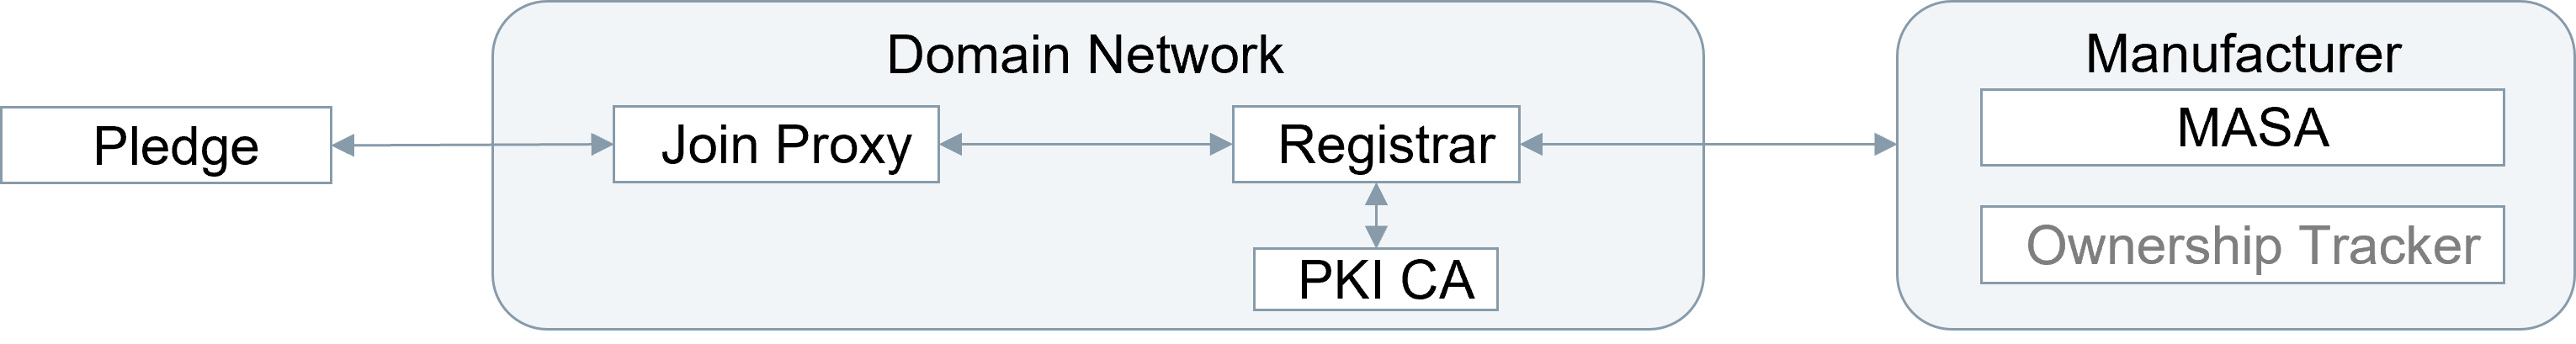
\includegraphics[scale=0.4]{Images/brski-overview.png}
	\caption{BRSKI Architecture.}
	\label{brski-architecture}
\end{figure}

The network domain is the domain of the alleged new owner of the device, i.e the network that is expecting the device to be connected to it. The domain is a network of entities who share a common local trust anchor. 
It incorporates a \gls{pki} to govern the issuance of digital certificates to provide unique digital identifiers for clients and establish end-to-end security. 
\par
A join proxy is another component of the domain. It helps with the discovery of pledges that intend to join the network. In addition, it is responsible for discovering the domain registrar(s) and determining the proxy mechanisms supported by the registrar and utilizing the lowest impact mechanism.
Pledge discovery methods can be classified into passive and active methods. 
GRASP flooding \cite{rfc8990} is a pledge passive discovery method for autonomic networks \cite{kephart2003vision}. It is short for GeneRic Autonomic Signaling Protocol. It is used for signaling between autonomic service agents. GRASP provides discovery, flooding, synchronization, and negotiation functionalities for the technical objectives through respective GRASP messages. Pledge discovery via GRASP multicast flooding is the normative and mandatory method for \gls{brski}.
On the other hand, DNS-based Service Discovery \cite{rfc6763} over Multicast DNS \cite{rfc6762} as well as DHCP \cite{rfc2131} are pledge active discovery methods. They can be used as secondary discovery methods in parallel to GRASP.
Moreover, A proxy provides HTTPS connectivity and forwards messages without examination between a pledge and a registrar in the network, and without interfering with the protocol messages.
\par
A pledge is an unconfigured device attempting to join the network domain. Its goal is to be securely bootstrapped in a zero-touch fashion. To achieve this goal, the pledge establishes a TLS connection with one or more of the domain's registrars through the domain's proxy. It is necessary for the pledge and the registrar to establish mutual authentication. A manufacturer installed \gls{idevid} is used for pledge authentication to the domain's registrar. It is installed during the manufacturing process and includes certificates signed by the manufacturer and unique identifiers that represent the pledge, in addition to, the pledge unique serial number given by the manufacturer. It is recommended that The provided certificates are used for authentication with the registrar and the signing of voucher requests. The unique serial number is used in vouchers and voucher requests to ensure linkability. 
\par
A registrar is an element of the domain that is responsible to carry out the bootstrap process for the pledge. Also, it can be considered as the \gls{ra} for the domain's \gls{pki}. A domain can have one or more registrars which all have to be recognized by the domain proxy. If the pledge is capable to concurrently connect to multiple registrars, it is advisable to do so as this protects against a malicious proxy attempting a \gls{dos} attack like Slowloris.
\par
A manufacturer is the entity that produced the device and set up its initial configuration (IDevID). It provides two distinct services: the \gls{masa} service and ownership tracking and validation.
MASA can be a third party service that signs the vouchers issued for the bootstrapping process. It is also responsible for providing a repository for audit-log information of bootstrapping events. The service is contacted each time a pledge performs a zero-touch bootstrap in an attempt to enroll into a domain. It takes the decision whether or not issue the voucher according to the MASA policy. Voucher issuance could be done blindly at the lowest security level or it could be tightly bound to the sales channel that verifies the actual ownership of the domain. Hence, the manufacturer can provide protection against stolen devices or illegitimate resale of devices by declining voucher issuance to the suspected pledge.
\par
Ownership tracking and validation is an optional manufacturer service. It is supposed to log all claim attempts and to know which device is owned by which domain and provide such information to registrars. A verified log entry indicates that the pledge was issued a voucher as a result of positive verification of ownership.

\subsection{Protocol Details}
This section describes the message sequence of BRSKI illustrated in figure \ref{brski-protocol} and elaborates on content of the exchanged messages. The numbering sequence referenced through this section refers to the message numbers in figure \ref{brski-protocol}.

\begin{figure}[htbp]
	\centering
	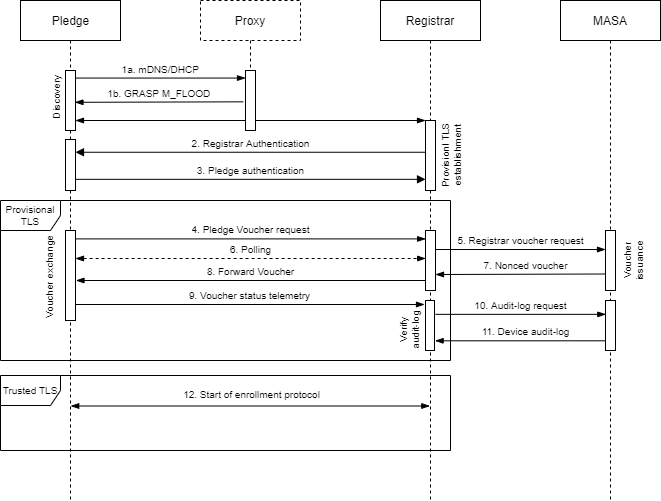
\includegraphics[scale=0.4]{Images/brski-architecture.png}
	\caption{A successful BRSKI protocol run.}
	\label{brski-protocol}
\end{figure}

\begin{itemize}
	\item \textit{Message 1a, 1b (Discovery phase):} It is the first phase of the protocol where the pledge identifies the domain proxy. This can be performed by a pledge initiated mechanism as in message (1a) or via a proxy initiated mechanism as in message (1b). After successful discovery, the pledge can address a domain registrar through the proxy. A proxy does not assume any specific TLS version.

	\item \textit{Message 2, 3 (Provisional TLS establishment):} The pledge attempts to establish a TLS channel with each discovered registrar to ensure End-to-End security. The pledge must not use any TLS version lower than TLS 1.2, while TLS 1.3 is the encouraged version to be used. To establish the channel, mutual authentication has to be performed.
	At first, in message (2), the pledge receives the registrar's server certificate. However, the pledge does not posses any trust anchors to verify it yet. Therefore, the pledge accepts the registrar's certificate provisionally.
	Next in message (3), the pledge is authenticated via the installed IDevID. The registrar must be able to verify the provided certificate, however the distribution of the trust anchors for this task is out-of-scope of BRSKI.
	Meaning, the information received by the pledge must be untrusted, although it is in a TLS channel, till a trusted trust anchor to verify the certificate is received. 

	\item \textit{Message 4:} Having established a secure provisional TLS channel, the pledge initiates the voucher exchange by sending a pledge voucher request to the registrar in message (4). The request must contain a unique nonce per bootstrapping attempt to protect against replay attacks. Also, the request contains the `proximity-registrar-cert' and the pledge serial number.
	The `proximity-registrar-cert' is the \gls{ee} certificate of the registrar which is also used to establish the provisional TLS channel. Pledge serial number is a manufacturer defined unique identifier for each device. It is different from the IDevID certificate serial number. Since not all devices have a real-time clock, depending on the device capabilities, the request is recommended to have the 'created-on' value. Finally, the request must be signed using the pledge's IDevID certificate.
	\par
	The registrar authorizes the pledge based on the authenticated information presented in the pledge's IDevID and the registrar's policy. The policy can be either to allow any device from a specific vendor, to allow any device of a specific type, or to allow a specific type of devices from a specific vendor.
	
	\item \textit{BRSKI-MASA TLS channel:} The registrar initiates a TLS 1.2 or newer channel with the MASA where all subsequent communication between the two parties occur within this secure channel. The MASA URL is obtained from the pledge IDevID, as mentioned earlier. To authenticate the MASA, the registrar should be configurable with trust anchors on a per vendor MASA basis as part of the sales process. Moreover, the registrar should also support client authentication mechanisms such as TLS client certificate, HTTP Basic, Digest, or \gls{scram}; however TLS Client Certificate based authentication is the recommended method.
	
	\item \textit{Message 5:} After obtaining the pledge's voucher request, the registrar constructs a registrar voucher request that is sent to the MASA to obtain a voucher for the pledge. The registrar voucher request is a JSON document that is signed using a CMS structure. The JSON document encapsulates the pledge voucher request CMS object that was sent to the registrar and is referred to as `prior-signed-voucher-request'. Moreover, the request contains the `created-on' field which holds the timestamp the request was formed on. In addition, it consists of other fields which relate to the pledge request like the pledge serial number, the nonce used produced by the pledge and used in the pledge request, and `idevid-issuer' field which holds the issuer value of the pledge IDevID certificate. The registrar includes some certificates in the registrar voucher request CMS object as well. Those certificates are used by the MASA to be pinned into the voucher to be later used by the pledge as a trust anchor for authenticating the domain registrar. Therefore, the certificates enclosed by the registrar in the request have to be part of the chain it wishes the MASA to pin in the voucher. Hence the specificity of the attached certificates is considerably significant. A `pinned-domain-cert' can be as specific as the registrar's TLS \gls{ee} certificate. On the other hand, if it is as general as a public webPKI \gls{ca} it could permit any entity that possess a certificate issued by that authority to claim ownership of the device.
	\par
	On the other hand, the pledge might not be available at the time of deployment to send a pledge voucher request, or the registrar speculates to not being able to reach the MASA at the time of deployment where the pledge will be available. Such use cases justify the need for nonceless registrar voucher request. In these cases, the previous message (4) would not exist. To formulate this request, the registrar has to acquire the pledge's serial number and IDevID issuer, however, they are obtained through out-of-band means. Subsequently, the nonce field of the request is omitted.
	
	\item \textit{Phase 6 (Polling)}: Before processing the pledge's request, the registrar may send the pledge an HTTP 202 response message which indicates that the request received earlier has been accepted for processing however processing is not yet complete. This response initiates a polling phase between the pledge and the registrar. A ``Retry-After" field is specified within the headers of the registrar's response that indicates the minimum time for the pledge to wait before asking for a response for the voucher request sent earlier. After the specified waiting time, the pledge polls the response by resending the exact same request and must not change the nonce nor sign a new voucher request. If the pledge is simultaneously trying to bootstrap itself with several registrars of the network, it can be overwhelming for the pledge to keep track of all the ``Retry-After" times. Therefore, a pledge may ignore the specified interval and follow a hard-coded ``Retry-After" interval. A pledge should be able to hold the retry state for a maximum of 4 days.
	
	\item \textit{Message 7:} upon receiving the voucher request, the MASA performs a set of checks to decide weather to issue the requested voucher. Given the fact that vouchers have a short lifetime, the request may be from a registrar that has been issued a voucher previously, i.e a voucher renewal request. In this case, the request should be automatically authorized by the MASA.
	\par
	 The MASA extracts the certificate chain attached in the signed CMS object. If the domain CA is unknown to the MASA it is considered as a temporary trust anchor as the intention is not to authenticate the message rather to establish consistency of the domain PKI. According to the MASA's policy, it decides which certificate of the chain supplied by the registrar it chooses to pin. It may be the farthest certificate of the chain, or it may be as close as the \gls{ee} TLS certificate of the registrar. If revocation information is available for that certificate, it must be checked by the MASA to prevent issuance of new or renewed vouchers to unauthorized registrars. Next, the CMS signature is validated using the domain's CA extracted from the voucher request. Also, the signing certificate is verified to contain the `id-kp-cmcRA' Extended Key Usage. This ensures that the signer is an entity that is authorized to be a registrar of the domain. Hence, assures domains that a MASA only accepts requests from domain registrars. 
	 \par
	 In case of nonceless requests, It is mandatory for the MASA to authenticate the registrar. The decision to issue a noncless voucher is taken according to the MASA policy that is out of scope.
	 \par 
	 In case of nonced voucher requests, the MASA verifies that the `prior-signed-voucher-request', enclosed in the registrar request, contains a `proximity-registrar-cert' that is coherent to the certificate used to sign the registrar voucher request. Moreover, the nonce is verified to be consistent between the registrar voucher request and the `prior-signed-voucher-request'.
	 \par
	 Subsequent to a successful validation of the request, the MASA responds with an issued voucher in message (6). Any issued voucher by the MASA is recorded in the audit-log. Otherwise if a problem occurs, a response with the appropriate http signaling as described in \cite{brski}. For example, a 403 status code response if the voucher request is not signed correctly, or a 406 status code response if the requested voucher type or algorithms cannot be issued due to the MASA's awareness that such pledge is not capable of processing them.
	 
	\item \textit{Message 8:} The registrar evaluates the received voucher solely for transparency and future audit-log verification. The received voucher is forwarded to the pledge without any interference or modification from the registrar.

	\item \textit{Message 9:}
 	 After the pledge successfully receives a voucher, the pledge must indicate its status regarding the voucher to the domain. This occurs by sending a status message to the registrar. The pledge decides weather to accept the voucher or not through the voucher validation process. If acceptable, the message should contain the version of BRSKI and a boolean status field to indicate the acceptance status. In case of an unacceptable voucher or a failure, the pledge is expected to fail gracefully. The message should contain a Reason field with a string commenting on the cause. Nevertheless, the Reason should not be excessively descriptive as it may be sent to an unauthenticated and potentially malicious registrar.
	 \par
	 Bearing the voucher, the pledge verifies its validity. It verifies the signature using the manufacturer installed MASA trust anchor. It verifies also that the serial number enclosed in the voucher matches its own. For nonced vouchers, the pledge verifies the voucher nonce corresponds to the nonce it sent earlier in the voucher request. However nonceless vouchers can be accepted according to pledge local policy. The pledge can be configured to always accept nonceless vouchers to realize the use case where the MASA is unreachable at the time of pledge deployment.
	 \par
 	 A pledge could be operating in other similar security reduced mode that skip voucher validation in favor of offline or emergency touch-based deployment bootstrapping procedures. For example, \gls{tofu} or physical presence methods such as the use of serial console or depressing a physical button during bootstrapping. However, \gls{tofu} must not be available unless a hardware-assisted \gls{nea} is supported. Meanwhile, it is only recommended for other methods of skipping voucher validation. This recommendation serves as a prevention against unintended use of offline methods when autonomic methods fail or are unavailable.
	 \par
	 Upon successful verification of the voucher, the voucher's pinned-domain-cert should be considered by the pledge as a trust anchor. The current provisional TLS connection between the pledge and the registrar is evaluated using the obtained trust anchor. The pledge verifies the registrar's TLS server certificate using the trust anchor's public key. If the registrar's credentials could be verified, either by directly matching the server certificate or through verifying a higher certificate in its chain, the pledge trust the TLS connection and it is not considered provisional any further.
	 
	\item \textit{Message 10:} After receiving the pledge status telemetry message, the registrar requests the MASA audit-log from the MASA. The log data helps the registrar make a knowledgeable decision regarding further proceeding of the bootstrapping process. The decision making criteria is based upon the security requirements of the registrar domain. Hence, the criteria is out of the protocol's scope.
	The request content is the exact same registrar voucher-request sent earlier to the MASA, but is directed through a different URI specific for requesting the audit log, which is ``/.well-known/brski/requestauditlog". Reusing the same message minimizes the required cryptographic and message operations on both ends. The registrar may reuse the cached voucher request and the MASA may take advantage of its internal state to correlate the message with the already verified request averting additional operations.
	
	\item \textit{Message 11:} 
	A MASA can infer the proper pledge log to be prepared from the ``idevid-issuer" and the ``serial-number" information included in the received request of the previous message. Instead of immediately responding with the audit-log, the MASA can a HTTP 201 ``Created" response with a URL in the ``Location" header field redirecting to actual audit-log. The response log is a JSON format document consisting of all the log entries associated with the pledge. Nevertheless, a MASA that sends out URLS has to ensure they are unpredictable to avoid enumeration attacks against device audit-logs.
	\par
	The log format structure consists of several entries: ``version", ``events", and ``truncation". ``version" is an integer value representing the log format version. ``events" is an array of event objects that are associated to the device. 
	Each of the event objects is comprised of a set of entries. The ``date" entry represents the event's timestamp in the format according to \cite{rfc3339}. 
	The ``domainID" is a unique identifier for the domain's registrar that encodes the pinned-domain-cert's SubjectKeyIdentifier or SPKI fingerprint in base64. A ``nonce", if exists, is a base64 encoding of the same nonce used in the voucher request and issued voucher. If it is a nonceless voucher, then the field should preferably be set to null rather than omitting it. 
	The ``assertion" field indicates the level of verification with which the MASA issued the voucher. It can have one of three values: ``verified", ``logged", and ``proximity"; the latter being the one supported by this protocol.
	``truncated" field shows the number of event truncations for the specified domainID.
	Lastly, since audit-logs can be arbitrarily large, duplicated or old entries may be truncated as an optimization for the log structure. The ``truncation" entry contains meta-information about truncated entries such as ``nonced duplicates", ``nonced duplicates", and ``arbitrary".
	\par
	On the registrar side, the received audit-log is vetted for discrepancies and unexpected behavior like the pledge previously imprinting to an unexpected domain or whether a certain domain possesses a nonceless voucher and can reset the device anytime. If the registrar's audit-log verification is successful, then the bootstrapping process is complete.
	
	\item \textit{Message 12:} 
	At this point, the pledge has a trust anchor allowing it to verify the registrar, as well as a trusted TLS channel between them. Therefore the environment is suitable to start a certificate enrollment protocol after which the pledge obtains digital certificates that authenticate it to the domain and authorize it to utilize the relevant domain services.
	\par
	BRSKI is described as an extension for \gls{est} that provides automated proposal instead of the originally manual authentication method that relies on the intervention of a human user. Hence it is recommended for a pledge to use EST following BRSKI as a certificate enrollment protocol as it is considered a harmonious integration.
	\par 
	Nonetheless, the succeeding certificate enrollment protocol is not limited to \gls{est}, however, a variety of certificate enrollment protocols can be used. Using \gls{est} is an example of a pull model where the EST server is the protocol initiating party. As an example of the push model architecture, \gls{cmp} can be used as the certificate enrollment protocol since the \gls{ee} is the initiating party of the protocol. 
	

\end{itemize}











%sztp section
\section{\acrfull*{sztp}}

\section{Protocols Comparison}

\chapter{Post-Compromise Security} \label{ch:postcomp}
%Intro
Intro\\compromise window\\
\section{\acrfull*{x3dh}}
\textbf{\LARGE \# FIXME intro \#}
\label{ch:x3dh}

Key establishment protocols are utilized by communicating parties to establish shared secrets, in some cases, with the aid of a trusted third party \cite{handbookOfAppliedCrypto}. As per \cite{handbookOfAppliedCrypto}, key agreement is a key establishment technique in which a shared secret is derived by parties as a function of information related to them, such that the secret in not predeterminable nor deducable by outsiders.
\par
The Security of protocols is required to be proven to avoid the devastating effects of malicious attacks. Therefore, verification of security protocols is a vital process. Verification is proving that a protocol model is secure by achieving a set of security goals. There are various model checking tools that provide verification.
\par
\gls{x3dh} is a key agreement protocol intended for asynchronous settings \cite{x3dh}. The protocol can establish a shared secret between two parties in an environment where it is recurring that one of the parties is offline and the other wishes to send it an encrypted message. Also, X3DH provides the desired feature of forward secrecy. 
\par
This chapter discusses the \gls{x3dh} key agreement protocol \cite{x3dh} and verifies the security of the protocol using \gls{ofmc} \cite{ofmc}.
\subsection{Protocol Overview}
\subsubsection{Roles}
A protocol run involves three roles: Alice, Bob, and a server. In this description, Alice wants to send an encrypted message to Bob. Bob is the party that may be offline at that time and wishes to enable other parties to derive a shared secret with it, through a set of public information Bob publishes. The server is responsible for 1. storing the public information published by Bob, and 2. storing messages for offline parties till they are fetched. The server is not trusted, however, it is assumed to be resilient against DoS. % more details.
\subsubsection{Keys}
\gls{x3dh} utilizes Elliptic Curve asymmetric key pairs. All keys used in a protocol run must all be derived from the same curve, either $X25519$ or $X448$. Each role has to have a set of keys to run the protocol. Table \ref{tab:x3dhkeys} lists the public keys required for each role. Note that for each public key, there exists a corresponding private key at its owner.

\begin{table}
	\centering
	\begin{tabular}{|c||c|c|}
		
		\hline
		Owning Role & Notation				 & Description 			  \\\hline
		\multirow{2}{*}{Alice} & IK\textsubscript{A} 	 & Long-term identity Key \\
		& EK\textsubscript{A} 	 & Ephemeral Key 		  \\\hline
		\multirow{3}{*}{Bob}  & IK\textsubscript{B} 	 & Identity Key 		  \\
		& SPK\textsubscript{B} 	 & Signed Prekey 		  \\
		& OPK\textsubscript{B} 	 & one-time Prekey 		  \\ \hline
		
	\end{tabular}
	\caption{\gls{x3dh} keys.}
	\label{tab:x3dhkeys}
\end{table}

\begin{itemize}
	\item \textit{Identity keys}: They are long-term public keys known by their corresponding parties before the protocol run.
	\item \textit{Ephemeral Keys}: This type of key pair is freshly generated within the protocol run.
	\item \textit{Signed Prekey}: This key pair is generated and signed by its owner. The prekey is signed using the private identity key. The life time of this key pair is shorter than that of the identity key pairs as it is updated periodically by its owner. The corresponding role owns only one signed prekey at a time.
	\item \textit{One-time Prekey}: The corresponding role generates multiple one-time prekey. Each is can be used for only one protocol run. The responsible party is supposed to supply the these keys as they should not run out. In case there are not any keys left, the protocol can run, however without one of the \gls{dh} operations as explained in section 2.3.
\end{itemize}

\subsubsection{A Protocol Run}
%\subsubsubsection{Registration phase} 
At first, the protocol starts with a registration phase. Initially, The party acting in the role of Bob publishes to server the public information required to run the protocol with it by any party acting as Alice. Bob publishes his $ IK_{B} $, $ SPK_{B} $, Bob's prekey signature, and a set of $ OPK_{B} $.

\par
%\subsubsubsection{The initial message}
Next, the inline party sends the initiates the protocol by sending the first message. First of all, Alice fetches a \textit{prekey bundle} from the server to contact Bob. This bundle contains:
\begin{itemize}
%	\setlength\itemsep{-0.3em}
	\item Bob's Identity key $ IK_{B} $.
	\item Bob's signed prekey $ SPK_{B} $.
	\item Bob's prekey signature.
	\item If exists, a one-time prekey $ OPK_{B} $. The server deletes the $ OPK_{B} $ sent to Alice.
\end{itemize}

Before proceeding, Alice verifies the prekey signature and quits the protocol if the verification fails.
At this point, Alice has enough information from Bob to deduce a shared secret. Alice generates her Ephemeral key pair $ EK_{A} $. With the set of available keys, Alice performs three \gls{dh} operations which are extended to four if a $ OPK_{B} $ is available. Figure \ref{fig:x3dh} presents the relation between the keys.

\begin{itemize}	
\item $ DH1 = DH(IK_{A_{p}} \footnote{\textit{p} indicates the private key of the key pair.}, SPK_{B}) $
\item $ DH2 = DH(EK_{A_{p}}, IK_{B}) $
\item $ DH3 = DH(EK_{A_{p}}, SPK_{B}) $
\item \textcolor{darkgray}{$ DH4 = DH(EK_{A_{p}}, OPK_{B}) $}
\end{itemize}

\begin{figure}[htbp]
	\centering
	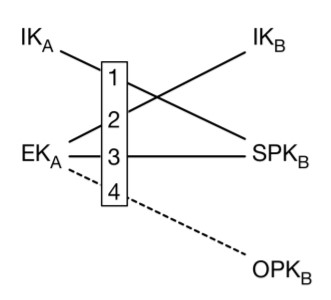
\includegraphics[width=0.4\linewidth]{images/X3dh}
	\caption{\gls{x3dh} operations \cite{x3dh}.}
	\label{fig:x3dh}
\end{figure}

The \gls{dh} outputs are fed into a \gls{kdf} to generate the shared secret $ SK $. Next, Alice deletes her $ EK_{A_{p}}$ and all \gls{dh} outputs for forward secrecy. At this moment, Alice is ready to send the initial message with the content encrypted using $ SK $. The initial message from Alice to Bob has to have enough information for Bob to generate the same $ SK $.
The initial message contains:
\begin{itemize}
%	\setlength\itemsep {-0.3em}
	\item $ IK_{A} $
	\item $ EK_{A} $
	\item Identifiers of Bob's prekeys used by Alice
	\item An initial ciphertext. The ciphertext can be used as an initial message for a post-X3DH communication protocol, e.g. Double Ratchet algorithm.
\end{itemize}

%\subsubsubsection{Bob's $ SK $ Derivation}
Upon receiving the initial message, Bob attempts to derive the $ SK $.
Using the key identifiers sent by Alice, Bob loads the private keys corresponding to the public keys Alice used. In combination with the keys $ IK_{A} $ and $ EK_{A} $ Alice sent, Bob can compute the same $ SK $ by doing the three (or four) \gls{dh} operations.
\par
Next, Bob attempts to decrypt the ciphertext. If the message is successfully decrypted to the expected format, e.g. the format of the first message of the post-X3DH protocol, then the protocol run was successful. Otherwise, Bob aborts the protocol and discards the $ SK $.

\subsubsection{Security Considerations}
%\subsubsubsection{Authentication}
Authentication is essential for both parties to guarantee the identity of who they are communicating with. Thus, Alice and Bob must authenticate the keys $ IK_{A} $ and $ IK_{B} $. However, the protocol specification does not discuss authentication methods.
\par
%\subsubsubsection{Protocol Replay}
The one-time prekey used in the fourth and optional \gls{dh} calculation is for protection against replay attacks as they ensure freshness of the protocol run. Absence of a one-time prekey could lead a replayed message to be accepted by Bob believing that Alice had sent it in the current protocol run.
\par
%\subsubsubsection{Server Trust}
A server can be a cause of attacks if malicious. It can carry out a Denial of Service attack if it refuses to forward the messages. It can deliberately not distribute one-time prekeys, exposing the protocol to replay attacks. Also, one party can drain all the one-time prekeys, if the server is not attentive to such action, leading to replay attacks.

\subsection{OFMC Verification}
This section aims at formally verifying the \gls{x3dh} protocol using the automated verification tool \gls{ofmc}. Briefly, \gls{ofmc} uses the clear and declarative modeling language $AnB$. The goal of the tool is verify the security of the modeled protocol, under an intruder model, in a fashion similar to deciding whether a mathematical statement is true or false. The intruder model is based on the famous Dolev-Yao model \cite{dolev1983security}. The intruder is assumed to control the network. Therefore, the network should not be relied on for any protection guarantees. Furthermore, the intruder is assumed to be knowledgeable to all cryptographic primitive. Lastly, \gls{ofmc} does not rule out the possibility that the protocol participants can be dishonest.

Presented in listing \ref{model} the code for modeling our variant of a secure \gls{x3dh} protocol under the Dolev-Yao intruder model in \gls{ofmc} using the \textit{AnB} language.

\lstinputlisting[numbers=left,          
numberblanklines=false, breaklines=true, columns=fullflexible,
frame=single,
breaklines=true,
postbreak=\mbox{\textcolor{red}{$\hookrightarrow$}\space},
caption={X3DH \gls{ofmc} Model},captionpos=b, label={model}]{code/x3dh.anb}

\subsubsection{Types section} 
Here, the parameters of the protocol are defined, e.g. variables, constants, roles, etc. Line 4 defines the participants of the protocol of type \textbf{Agent}.
\begin{itemize}
	\item $A$ and $B$: Variables indicating Alice and Bob. A variable may be dishonest in an \gls{ofmc} protocol run.
	\item $s$: Constant indicating the server. Constants act as trusted third parties.
\end{itemize}
\par
Line 5 defines the functions of the protocol.
\begin{itemize}
	\item $kdf$: Key derivation function.
	\item $pk$: A function to model asymmetric key pairs. A public key for Alice is modeled as $pk(A)$ and the corresponding private key is computed using the internal function $inv()$ as follows $inv(pk(A))$.
	\item $ik$: models the private component of the identity key of a party for the \gls{dh} calculations.
\end{itemize}
	Alice and Bob have long-term signing keys modeled by the function $pk()$ and long-term identity keys modeled by the function $ik()$.
	\par
Line 6 defines the numbers used in the protocol. Lower-case numbers are constants, while upper-case numbers are random and freshly generated during a protocol run. Some private components of keys are modeled as numbers as they are required to be freshly generated during a protocol run which can not be done using functions.
\begin{itemize}
	\item $g$: Public prime base for \gls{dh} calculations.
	\item $NA$: Alice's Nonce.
	\item $EKA$: The private component of Alice's Ephemeral key.
	\item $OTP$: The One-time prekey's private component.
	\item $PREKEY$: the prekey's private component.
	\item $MSG1$ and $MSG2$: Random numbers used as placeholders for random and fresh messages.
\end{itemize}

\subsubsection{Knowledge section}
This section of the model defines what knowledge is initially known to each party before the protocol starts. Line 9 defines Alice's knowledge which contains, in addition to the previously defined parameters, Alice's certificate modeled as $\{A, pk(A)\}inv(pk(s))$. This translates to Alice's identity $A$ and Alice's public key $pk(A)$ are signed using the servers private key $inv(pk(s))$. 

Line 15 holds a $where$ clause that strictly defines $A$ and $B$ as different parties to avoid the scenario where $A$ or $B$ talk to itself.
\subsubsection{Actions section}
The Actions section states the protocol's message sequence between the participating parties for a successful protocol run. Throughout this section messages are referred to according to their line number, e.g message 19 is the message in line number 19 of the model code.
\par
Message 19 represents the registration phase where Bob publishes his public information to the server. The whole message is encrypted for authenticity by the server's public key $pk(s)$. The message contains the following:
\begin{itemize}
	\item $exp(g,Z)$: The public \gls{dh} key of the corresponding private key Z. As known in \gls{dh}, the public key of a party is of the form $g^{Z}\ mod\ p$. For simplicity, \gls{ofmc} omits the prime modulus operation $mod\ p$. Hence, it is needed to only model the public key $g^{Z}$ by using the \gls{ofmc} modulus exponentiation function $exp(g,Z)$.
	\item $\{exp(g,PREKEY)\}inv(pk(B))$: The prekey of Bob signed by Bob's signing key.
\end{itemize}

\par
Message 21 is not an actual part of the protocol, however, it is included for the sake of modeling the protocol with the chosen tool. This is because of the asynchronous communication model of \gls{ofmc} and the strands concept \cite{ofmcTut}.
\par 
In message 23, Alice requests to fetch from the server a key bundle to communicate with Bob. A nonce $NA$ is attached for freshness.
\par
Message 25 is the server's response to Alice's key bundle request. The message contains the requested key bundle required to communicate with Bob, as well as Alice's nonce. The whole message is integrity protected by the server's signature.
\par
Message 27 represents the initial message from Alice to Bob. It is composed of the following:
\begin{itemize}
	\item (Line 27) Alice's certificate for authenticity.
	\item (Line 29) Bob's keys that Alice received from the server which will used to compute $SK$. All these keys are signed by Alice for integrity protection.
	\item (Line 31) The initial ciphertext encrypted by the symmetric key $SK$. Each output of the four \gls{dh} operations is input into the \gls{kdf} resulting in $SK$.
\end{itemize}
Message 38 is the last message of the protocol run. Here, Bob shows he is able to compute the same $SK$. 
\par
Notably, the modeling of the \gls{dh} operations in messages 27 and 38 is unnatural in contrast to how \gls{dh} is normally performed. Ordinarily, a \gls{dh} secret is the computation of $exp(g^{M},N)$ where $g^{M}$ is a public value and $N$ is a value private to the party performing the operation. According to exponential power of power rule $exp(g^{M},N)$ is equivalent to $exp(g^{N},M)$. Therefore, the other party should follow that intuition to result in the same secret output as its counterpart. 
It is observable that the symmetric key computation in message 27 is identical to the one in message 38.
The behavior for modeling $DH1$, $DH2$, and $DH3$ of message 27 is not expected, since Alice is explicitly using Bob's secrets ($PREKEY$ and $ik(B)$) in the \gls{dh} operations although they ought not be in Alice's knowledge.
This behavior is present in message 38, however, it is as it should be. To the reader, it could mean that Alice is knowledgeable of Bob's private keys, but, this is not the case. \gls{ofmc} aims to abstract the key creation process and makes it implicit for the tool users. The \gls{ofmc} compiler comprehends the exponential power of power property which enables it to automatically do the computation. Despite the previous clarification, $DH4$ computation contradicts what was mentioned. The $M$ and $N$ values for $DH4$ are swapped back to what would be naturally expected in comparison to the previous \gls{dh} operations of message 27. Although, this behavior is considered unnatural for message 38 as now Bob is considered to be using Alice's secret keys. However, this exceptional behavior for $DH4$ is a result of a limitation of \gls{ofmc}'s AnB-translator message composition heuristics, as the translator is not capable of recognizing four inversions in a row. Therefore, the exceptional behavior is a workaround to make the AnB-translator realize how to compose the message. This workaround was thankfully guided by Prof. M\"{o}dersheim, the composer of \gls{ofmc}.
\subsubsection{Goals section}
This section of the model lists the security goals which the protocol must achieve at the end of a run. There are two types of goals
\begin{itemize}
	\item Authenticity: When a party wants to make sure a certain message has been generated and sent by the other party. In this model, Alice and Bob authenticate each others' public keys. Bob authenticates the server on the keys he received in message 27 from Alice, to be sure that the keys are forwarded by Alice from the server without tampering.
	\item Secrecy: The requirement for a message to be secret only between some parties.
\end{itemize}
\input{Chapters/postCompromiseSecurity/x3dh/diff}
%\input{Chapters/postCompromiseSecurity/x3dh/result}





\section{Double Ratchet Algorithm}
\label{ch:dr}
The adoption of a ratchet mechanism is a popular mechanical approach that enables forward movement but inhibits backward movement. A ratchet-like action is performed in the context of secure communication by utilizing randomization in every state update, such that a compromised state is insufficient for the decryption of any subsequent transmission.
The Double Ratchet is a cryptographic asynchronous message exchange algorithm that provides high security to the communicating parties. Asynchronicity in this context refers to that even if the counterpart is not online, the messages should be conveyed (or the key exchange should be done) for a two-party conversation.
Furthermore, a significant design goal dubbed \gls{0rtt} is the ability to transfer payload data without necessitating online exchanges.
\par
The algorithm enables the exchange of encrypted messages based on a shared secret key between the two parties where each message is encrypted with its specific ephemeral key.
The double ratchet algorithm is a combination of two ratchet constructions which provide enhanced security properties.
The first outer ratchet is inherited from \gls{otr}'s asymmetric ratchet to benefit from its future secrecy property which is obtained through the use of ephemeral key exchanges. Coupled by an inner symmetric ratchet for forward secrecy, the algorithm was formed and was formerly named Axolotl Ratchet. Additionally, \gls{kdf} chains are a core concept of the algorithm. This section goes through the methodology of the algorithm, its features, and its security properties.

\subsection{\gls*{kdf} Chain}
As mentioned in section \ref{backgroung:kdf}, a \gls{kdf} is a function that takes as input a key and an input and produces a cryptographically secure hash output that is random-like.
A \gls{kdf} chain is a series of connected \gls{kdf}s where one output key of a \gls{kdf} is a \gls{kdf} key input of a succeeding \gls{kdf}. Figure \ref{fig:kdf-chain} shows an illustration for a \gls{kdf} chain that takes three external inputs and produces three random output keys.

\begin{figure}[hptb]
	\centering
	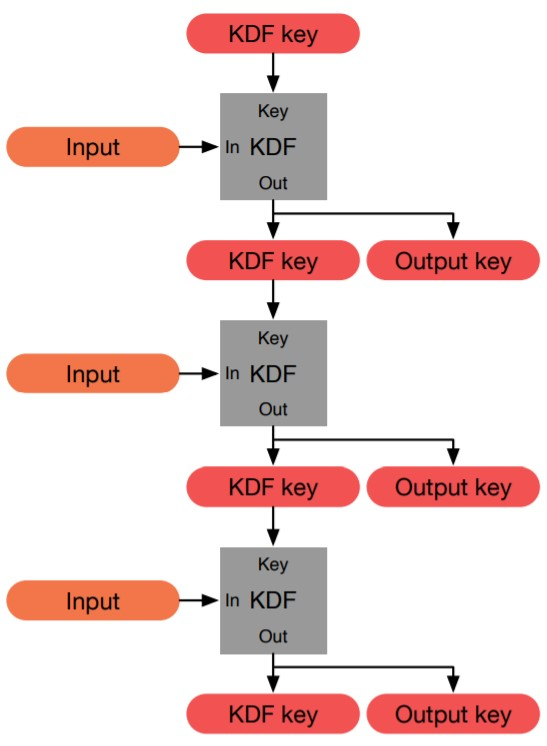
\includegraphics[scale=0.4]{Images/kdf-chain.jpg}
	\caption{A 3 input KDF chain \cite{dblRtcht}.}
	\label{fig:kdf-chain}
\end{figure}

The algorithm session has three \gls{kdf} chains: root chain, sending chain, and receiving chain. Each chain is advanced whenever its relevant ratchet performs a step. More details about ratchet steps and their relation to the \gls{kdf} chains are discussed in later sections.
\par
KDF chains have a set of characteristics \cite{dblRtcht}:
\begin{itemize}
	\item \textit{Resilience:} An adversary who does not know the KDF keys perceives the output keys as random. Even if the opponent has complete control over the KDF inputs, this is still valid.
	
	\item \textit{Forward secrecy:} An adversary who discovers the KDF key at some point in the future cannot distinguish between past output keys and random.
	
	\item \textit{Future secrecy:} If future inputs have contributed adequate randomness, future output keys seem random to an adversary who learns the KDF key at some point in the future.
\end{itemize}

\subsection{Symmetric-key Ratchet}
	
The sending and receiving chains are constructed of symmetric-key ratchets where Alice's sending chain is equivalent to Bob's receiving chain and vise versa. Essentially, a symmetric-key ratchet is a \gls{kdf} chain with a constant input through out the chain steps. However, unlike with random input, a constant input does not provide future secrecy.
\par
In a symmetric-key ratchet, the KDF key illustrated in figure \ref{fig:kdf-chain} is the chain key, while a KDF's output key is a unique message key. For a sending chain, a message key is used to encrypt the outgoing message. On the other side, a message key in the receiving chain is used to decrypt the incoming message. The process of calculating the next chain and message keys is an advance in the sending/receiving chain. This is referred to as a \textit{symmetric ratchet step}.
\par
Message keys are not re-introduced into the KDF chain, therefore, they can be discarded without proposing any security risk to earlier or later ratchet outputs. Also, it is possible to store message keys to handle out-of-order messages on the receiving end. Storing message keys introduce a risk to only their respective messages. However, a compromise of a chain key can lead to further compromise of future chain keys as future chain keys rely on previous ones.

\subsection{Diffie-Hellman Ratchet}
The \gls{dh} ratchet provides the future secrecy property. When paired with the symmetric ratchet, the combination addresses the symmetric ratchet lack of future secrecy. 
Each party generates a \gls{dh} key pair known as their \textit{ratchet key pair}. The parties exchange their public keys within message headers with which each can compute an equivalent \gls{dh} secret output using their own private key that is equivalent to the public key they sent. The process of generating a new \gls{dh} output when receiving a new public key is referred to as a \textit{\gls{dh} ratchet step}. Accordingly, a passive adversary that compromises one party's private key at a point in time is incapable of deducing the upcoming \gls{dh} outputs due to the use of newly generated key pair for each ratchet step.
\par
Next, we discuss an algorithm run where a \gls{dh} ratchet is advanced to create two different DH secret outputs between Alice and Bob. Bob is assumed to be the algorithm initiator. Figure \ref{fig:dh-bobRatchet} serves as visual aid for our discussion where we proceed in steps as labeled in the diagram.

\begin{figure}[hptb]
	\centering
	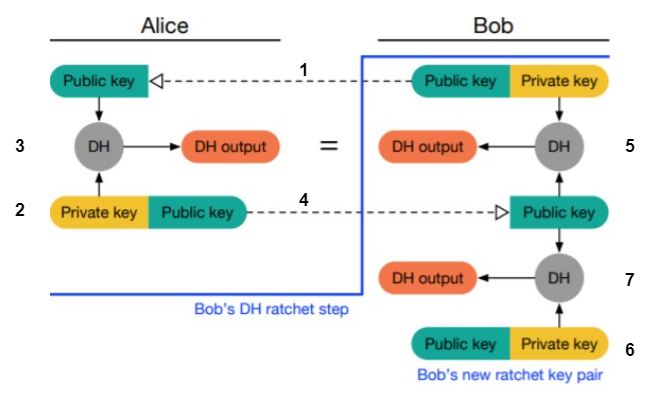
\includegraphics[scale=0.45]{Images/dr-bobRatchet.png}
	\caption{Bob \gls{dh} Ratchet step. Figure reproduced from \cite{dblRtcht}.}
	\label{fig:dh-bobRatchet}
\end{figure}

\begin{itemize}
	\item \textit{Step 1:} Bob generates his first ratchet key pair to send the initial message to Alice. The initial message contains Bob's public key. 
	
	\item \textit{Step 2:} Upon receiving Bob's public key, Alice generates her ratchet key pair.
	
	\item \textit{Step 3:} Alice performs a \gls{dh} calculation between her private key and Bob's public key generating her side of the DH output.
	
	\item \textit{Step 4:} Alice advertises to Bob her public portion of her ratchet key pair that was used to generate the DH output.
	
	\item \textit{Step 5:} After obtaining Alice's ratchet public key, Bob performs a DH calculation between it and his current ratchet private key resulting in Bob's copy of the shared DH output.
	
	\item \textit{Step 6:} Furthermore, Bob generates a new ratchet key pair to generate the next DH output.
	
	\item \textit{Step 7:} Bob performs a \gls{dh} calculation between hit new ratchet private key and Alice's public key generating a new DH output.
\end{itemize}
The steps described above are Bob's DH ratchet step as Bob was the initiator of the ratchet step by advertising his public key. Similarly, Alice's ratchet step starts by sending her public key to Bob and concludes after performing the same steps mentioned above but with the roles reversed.
\par
Linking the algorithm to the messaging context, the DH outputs represent the sending and receiving chains' root keys. 
Each party need to have two chains, sending and receiving chains. Alice's sending chain is equivalent to Bob's receiving chain and vice versa. As depicted in figure \ref{fig:dh-chains}, when a party receives a public key and computes its chain key using a private key that was generated prior to receiving the public, the resulting chain key is the receiving chain key. However, if they private key is generated after receiving the public key, the resulting key is the sending chain key. Simply put, if the public key is used in a DH operation upwards it produces a receiving chain key, while using it in a downwards DH operation generates a sending chain key.
\begin{figure}[hptb]
	\centering
	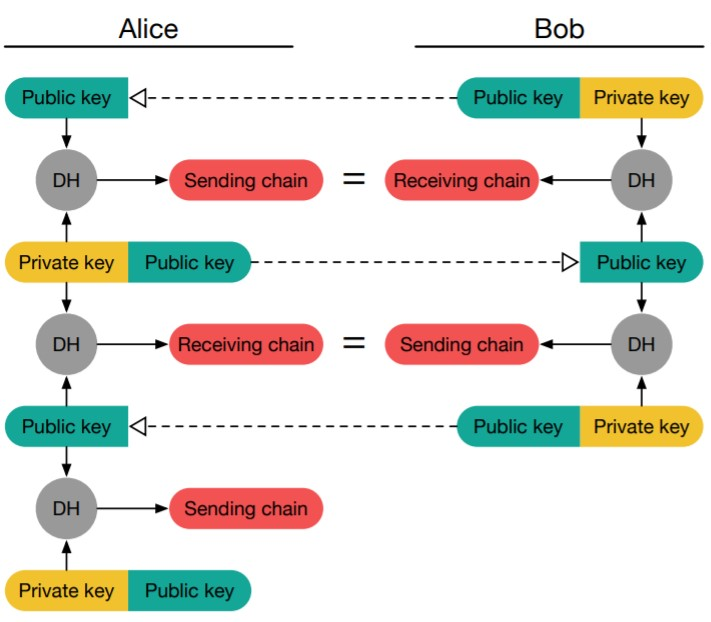
\includegraphics[scale=0.5]{Images/dh-chains.jpg}
	\caption{\gls{dh} chain keys generation \cite{dblRtcht}.}
	\label{fig:dh-chains}
\end{figure}
\par
However, the description so far is simplified. The algorithm is augmented by a KDF chain to improve resilience and future secrecy. The KDF chain key is a shared secret between both parties while the KDF inputs are the DH outputs from the DH ratchet. Every step through the KDF chain results in a new KDF root key and a sending/receiving chain root key. So a full DH ratchet step consists of updating the root KDF chain twice, generating both a sending and a receiving chain key. Figure \ref{fig:dh-ratchet_chain} illustrates a full DH ratchet step.

\begin{figure}[hptb]
	\centering
	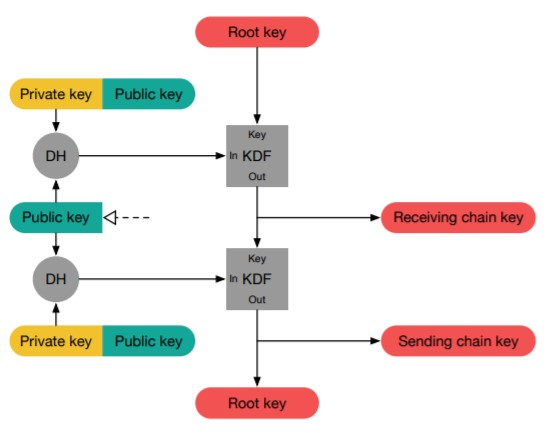
\includegraphics[scale=0.65]{Images/fullDHRatchetStep.jpg}
	\caption{A full \gls{dh} Ratchet step \cite{dblRtcht}.}
	\label{fig:dh-ratchet_chain}
\end{figure}

\subsection{Double Ratchet}
The double ratchet combines both the symmetric-key ratchet and the \gls{dh} ratchet to merge the security advantages provided by each. The outer ratchet is the \gls{dh} ratchet that provides ephemeral DH outputs which improve future secrecy. The DH outputs are fed as inputs to a KDF root chain lying between the outer and inner ratchets. It contributes to augmenting the security features by providing resilience and forward secrecy to the generated keys. The initial \gls{rk} for the KDF chain is a shared secret between the parties, e.g. an output of a key agreement protocol. The KDF chain outputs a new \gls{rk} for the next KDF and a new root \gls{ck} to create a new sending/receiving chain. Lastly the inner ratchet is the symmetric-key ratchet. Their root chain keys are the \gls{ck}s generated from the previous layer. They form the sending and receiving chains. When this ratchet is advanced it generates a new \gls{ck} and a message key. The \gls{ck} is used in the next KDF and the message key is used to encrypt or decrypt the message, depending on its respective chain. 
\par
Figure \ref{fig:AliceDR} serves as an example scenario for an algorithm run as it illustrates Alice's perspective of her double ratchet algorithm after a series of steps. 
\begin{figure}[hptb]
	\centering
	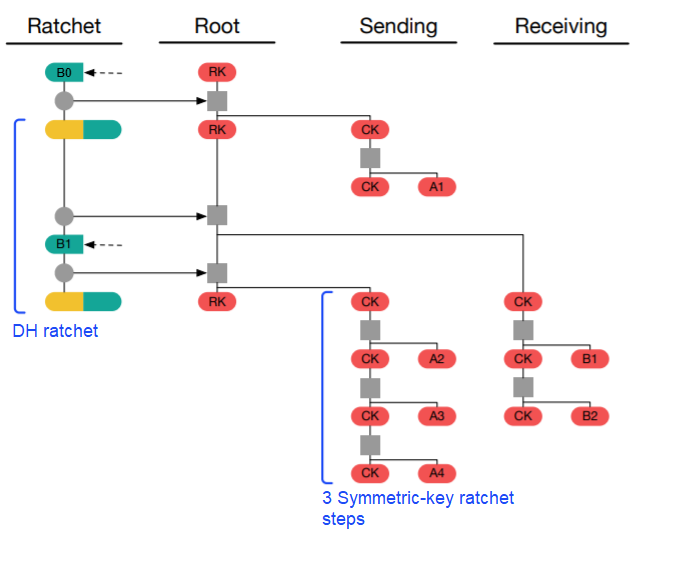
\includegraphics[scale=0.48]{Images/dr.png}
	\caption{Double ratchet from Alice's point of view. Figure reproduced from \cite{dblRtcht}.}
	\label{fig:AliceDR}
\end{figure}
The figure is split into four columns describing the aspects of the algorithm and how they are connected to each other. The first column represents the DH ratchet, the second shows the root KDF chain, and the last two depict the sending and receiving symmetric-key ratchets. Messages are denoted by the initial of the sender and the number of the message, e.g. $A1$ denotes Alice's first message. Keys follow the same abbreviation convention, e.g. $B1$ denotes Bob's first message key. Whether the key is a public key or a message key is represented by their highlighted color. Message keys are highlighted in red while public keys are highlighted in green.
\par
Alice is initialized by receiving the initial public key $B1$ which she uses to compute the input for the root KDF chain through a DH operation. Along with the pre-shared \gls{rk}, Alice computes a root \gls{ck} for her sending chain and a new \gls{rk}. Using the initial \gls{ck}, Alice creates a sending chain by performing a symmetric-key ratchet and producing a new \gls{ck} and a symmetric key $A1$ that she uses to encrypt her first message to Bob.
\par
Till this point, Alice is able to send encrypted messages to Bob as it had created her sending chains. However, she cannot decrypt Bob's messages as she has not yet created a receiving chain to produce the keys required to decrypt Bob's messages. As soon as Bob sends his next message with a new public key, Alice uses the public key $B1$ attached in the message header to step her DH ratchet. $B1$ is used in a DH operation with the previously created key pair to ultimately produce a root \gls{ck} to create a receiving chain. Alice performs a symmetric-key ratchet step of her receiving chain to produce the symmetric key $B1$ that decrypts the received message. Alice advances the same receiving chain to produce message keys to decrypt further message from Bob, e.g. $B2$, as long as the received messages do not contain new public keys in the message headers. However, since Alice received $B1$ and had to perform a full DH ratchet step, she has to generate a new ratchet key pair ultimately create a new sending chain. This implies if Alice wishes to send further encrypted message, she must use the new sending chain to generate the new message key. Thus in figure \ref{fig:AliceDR}, $A2$ is produced from the newly generated sending chain not the old one. As long as Alice has not received a new public key, she keeps advancing the sending chain to generate encryption keys for her outgoing messages, e.g. $A2$ and $A3$ in figure \ref{fig:AliceDR}.
\par
Parties should delete old keys as they no longer have a use. Keys are considered old if they have already been used and they are not going to be used in the future. For example, \gls{rk}s and \gls{ck}s which have already been input into KDFs or message keys that have already been used to encrypt/decrypt messages are considered old keys. Deleting old and useless keys is a good security practice as it prevents intruders from the possibility of recomputing keys that are dependent on those keys. Nevertheless, some keys can be saved to support additional functionalities such as handling out-of-order messages as explained in section \ref{oooMsgs}.

\subsubsection{Out-of-order Messages}\label{oooMsgs}
The Double ratchet algorithm can manage messages arriving out-of-order by simple additions to the message headers from the sender side. By including the message's index $N$ ($N=0$ for message 1) in the sending chain and the length $PN$ of the previous sending chain.
\par
If the sent message does not trigger a DH ratchet step on the receiver side, then the out-of-order message belongs to the current receiving chain of the receiver. The difference between $N$ and the actual receiving chain length is the number steps the receiver has to advance his receiving chain to obtain the message key required to decrypt the received message. The intermediate message keys for the skipped messages are stored in case they arrive later.
\par
On the other hand, if the message triggers a DH ratchet step, then the receiver uses the $PN$ to determine how many messages are skipped of his current receiving chain. The difference between the current length of the chain and $PN$ is the number of steps needed to advanced in the current chains and their produced message keys have to be saved. In this case, $N$ determines the number of skipped messages in the new receiving chain after advancing the DH ratchet. Likewise, the message keys for the skipped messages have to be saved supposing they are delayed for any reason.
\par
Implementation wise, the algorithm defines a \textit{MAX\_SKIP} constant that specifies the maximum number of message keys that should be saved for skipped messages. It should tolerate message loss or delay. However, it should not be too high that it allows for a malicious sender to trigger excessive recipient computation.
\subsubsection{Header Encryption}
As headers contain ratchet public keys as well as $PN$ and $N$ values, a passive attacker can infer the ordering of messages inside a session, or which messages belong to particular sessions. Therefore, encrypting message headers can reinforce messages security. Header encryption is achievable through each party having symmetric keys for both sending and receiving chains to encrypt or decrypt messages' headers. One chain header key is responsible for handling the header encryption of all messages within its respective chain. The header keys are integrated into the double ratchet algorithm as follows.
\par
Originally, Alice and Bob had only one pre-shared secret, the \gls{rk}. To integrate header encryption, the initial shared secrets need to include two unique \glspl{hk}, one for the sending chain and the other for the receiving chain (referred to as \acrfull*{nhk} in \cite{dblRtcht}). The initial \glspl{hk} are used for their respective first generated chains of the algorithm. To continuously obtain new \glspl{hk} for the newly generated chains which are a result of advancing the  DH ratchet, the root KDF chain is amended. Instead of generating only a new \gls{rk} and a new respective \gls{ck} with each step, the root chain is modified to additionally produce a \gls{nhk} of the relevant chain. A \gls{nhk} is a \gls{hk} that is to be used for the next chain of the same type that is to be generated after the next ratchet step. In this manner, at any point in time, before generating any chain of the algorithm, there exists already a header key to be used for that chain. When the chain is created, the \gls{nhk} becomes the current \gls{hk} for the chain and a new \gls{nhk} is generated simultaneously for the upcoming chain. Figure \ref{fig:DR-hk} shows an illustration of when \glspl{hk} are generated and how \gls{nhk} are used for the next chains.
\begin{figure}[hptb]
	\centering
	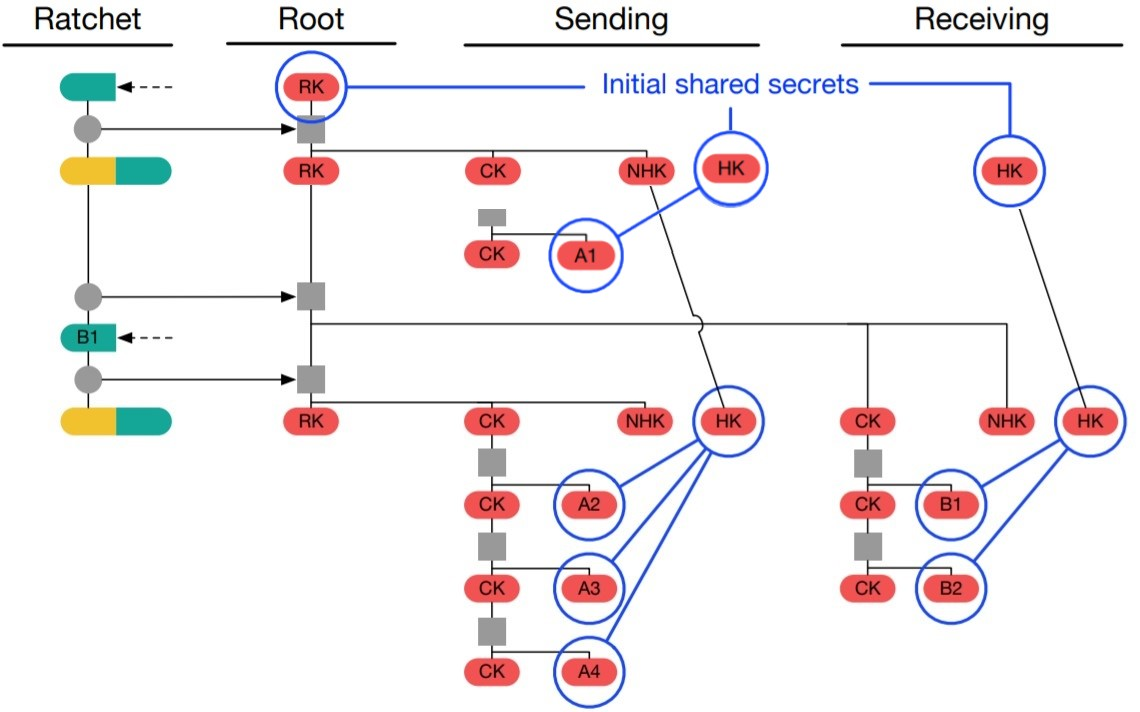
\includegraphics[scale=0.31]{Images/dr-hk.jpg}
	\caption{Usage of \glspl{hk} and \glspl{nhk} in the double ratchet algorithm. Figure reproduced from \cite{dblRtcht}.}
	\label{fig:DR-hk}
\end{figure}


\chapter{Implementation}
\label{ch:implementation}

Difference:\\
I don't create a new sending chain immediately in the DH ratchet step like the docs. I created on command. The docs mention that Bob can continue sending from the sending chain after Alice has created the equivalent receiving chain. However, when Alice creates the equivalent receiving chain she needs to create a new key pair. According to the implementation in the description, the new public key is automatically sent with the first message in the sending chain. This will lead to Bob automatically create a new sending chain and he has to use it rather than the old sending chain. thus, a contradiction. The mentioned scenario didn't assume the possibility of out-of-order messages yet. Therefore, I don't assume message delays.

\chapter{Discussion}
\label{ch:discussion}

\section{Secure Bootstrapping}
Both bootstrapping protocol presented in chapter \ref{ch:secureBootstrapping} provide very close core functionality in a similar fashion. However, in general, the protocols may not be directly adequate for all IoT constrained classes due to underlying PKI protocols which enforce expensive operations. However, with employing a lightweight PKI, like \cite{hoglund2020pki4iot}, or \cite{won2018decentralized}, the protocols may become more suitable for \gls{iot} setting. 
\par
Both protocols are applicable for any of the use cases presented in chapter \ref{ch:usecases}, however, a few design differences may make one protocol more desirable for a use case than the other. 
\begin{itemize}
	\item Unlike BRSKI, SZTP requires more communication between the owner and the manufacturer to exchange information and configuration before the start of the protocol in the Device Ordering and Owner Enrollment phase, especially if the owner is going to leverage the manufacturer hosted bootstrap server. This puts more burden on the manufacturer as they he has to configure the devices with extra information which may delay commissioning of devices. Such a delay may impose a disadvantage for scalable use cases such as the Industrial IoT use case as it can affect the agility of supply chain. On the other hand, on a smaller scale, such as the \gls{abc} use case, it may take some burden off the owner.
	
	\item SZTP can optionally host owner's specific device configuration and provision it along with other bootstrapping information. This feature can be useful for scalable use cases such as V2X communication and Industrial IoT as it speeds up transitioning the device into the operational phase. Nonetheless, for confidentiality critical systems such as \gls{abc}, it may not be advisable to have critical configuration hosted on third-party servers. Since, \gls{abc} devices are deployed on a limited scale, it is less necessary to use such a feature.
\end{itemize}

\section{Post-Compromise Security}
We argue that the protocols discussed are applicable in the setting of IoT.
First of all, the protocols offer desired secure communication properties, such as asynchronous authentication, non-repudiation (in our model), forward secrecy, and future secrecy.
Furthermore, the X3DH protocol does not impose any additional traffic overhead as it is a \gls{0rtt} protocol. Therefore, it can be used as the key agreement protocol in between IoT devices. However, the double ratchet algorithm adds a small overhead to the message header by including the DH public ratchet key in the headers.
\par
Nevertheless, handling out-of-order messages, as described by the algorithm, will cause a memory overhead, as the devices have to store lists of message keys. For constrained IoT devices, this is not suitable.
Furthermore, the double ratchet algorithm may introduce additional computational overhead. Since, for each DH ratchet step, a new key exchange operation occurs, the significance of the computational overhead is directly proportional to the frequency of performing a DH ratchet step. Therefore, we argue that it is a trade-off between the strength of provided security and the computational overhead. The use case decides this trade-off.
Reflecting on the defined use cases in chapter \ref{ch:usecases}:
\begin{itemize}
	\item For the \gls{abc} use case, since the security is critical, it may be preferable to perform a DH ratchet as frequent as with every message exchange. Since the \gls{abc} stations are stationary and not equipped with highly constrained IoT devices, we assume it can handle such a computational overhead.
	\item In the Industrial IoT setting, constrained IoT devices are constantly communicating with each other and with other services. Therefore, frequently performing a DH ratchet would not be efficient and will impose a great computational overhead. In such a use case, a DH ratchet can be performed based on a time interval or after a set number of messages.
	\item As mentioned earlier, V2X communication depends on three types of messages: broadcast, multicast, and unicast. For broadcast messages, the use of the double ratchet algorithm is not applicable as they are not encrypted. The double ratchet algorithm is not a proper choice for generating keys to protect messages using \gls{mac} as it has to set up sending chains with each receiver which is an infeasible process due to the arbitrary number of receivers. \gls{tesla}, described in section \ref{bg:tesla}, is a more suitable solution. Since our focus is on two party communication, multicast is out of scope. 
	Communication sessions between a vehicle and another entity will normally be short due to vehicles being usually in motion. Accordingly, the number of exchanged messages between the communicating parties will be small. Hence, even if a DH ratchet step is performed with every message, the computational overhead would still be limited.
\end{itemize}

\chapter{Conclusion}
\label{ch:conclusion}
The first goal of this thesis is to examine the significance of secure zero-touch bootstrapping of IoT devices. We analyze and present a comparison between two bootstrapping protocols: \gls{brski} and \gls{sztp}. 
Secondly, we aim to discuss the future secrecy of cryptographic keys in IoT through analyzing the \gls{x3dh} protocol and the double ratchet algorithm. In addition to use \gls{ofmc} to formally verify a model of a \gls{x3dh} protocol variant. Moreover, provide an implementation for the future secrecy related protocols.
Thirdly, we discuss the applicability of the mentioned protocols in IoT-related use cases.
Lastly, we aimed at conducting a comparative study between certificate enrollment protocols.

At first, we presented in chapter \ref{ch:background} an overview of different concepts and cryptographic primitives, as well as related work, which are a foundation for understanding the work presented through out the thesis. Next in chapter \ref{ch:usecases}, Three use cases are introduced: \acrfull{abc}, Industrial IoT, and V2X communication. For each use case, we further discuss the relevance of secure communication and the challenges it faces. In chapter \ref{ch:secureBootstrapping}, we first give a general overview of secure bootstrapping. Afterwards, for each of the zero-touch protocols, \gls{brski} and \gls{sztp}, we give an overview of the protocol architecture, in addition to explaining the execution details for each protocol to accomplish bootstrapping of a pledge. Moreover, we compare and contrast both protocols. Furthermore, in chapter \ref{ch:postcomp}, we discussed the post-compromise security property, aka future secrecy, in the realm of secure messaging and how it differs from forward secrecy. Also, we explain two protocols, which are part of the signal protocol, that work together to achieve desirable secure messaging properties ---in the context of two party communication only--- that include future secrecy, \gls{x3dh} and the double ratchet. For the \gls{x3dh}, we additionally use \gls{ofmc} to perform a formal verification for a model of the protocol. The model is a modified version from the original specification to guarantee its security under the \gls{ofmc} intruder model. Nevertheless, our variant scarifies the deniability property offered by the original protocol. For both protocols, we discuss their post-quantum security and other worked related to their formal verification. In chapter \ref{ch:implementation}, we present a demo implementation of the protocols discussed in chapter \ref{ch:postcomp}. Chapter \ref{ch:discussion} discusses the usage of the explained protocols in chapters \ref{ch:secureBootstrapping} and \ref{ch:postcomp} in the IoT world and the use cases defined earlier. Finally, we present a comparison of certificate enrollment protocols in appendix \ref{appendix-enrollment}. 

Although the thesis does not finally conclude the discussion of IoT security, we have shown how the mentioned bootstrapping protocols achieve their goal without manual input from the user during the process. Despite the highlighted differences, both protocols share a large set of functionalities.
Regarding X3DH protocol and the double ratchet algorithm, they are viable solutions and applicable to IoT and provide and enhance security in the proposed scenarios.

\newpage
\printbibliography

\appendix
% -- Appendix (optional)
\chapter{BRSKI vs. SZTP}\label{appendix-A}
\section{Terminology Comparison}
% Table generated by Excel2LaTeX from sheet 'Terminology comparison'
 \centering
 \begin{longtable}{|p{2cm}|p{4cm}|p{2cm}|p{4cm}|}
  \hline
  \rowcolor[rgb]{ .745, .804, .843}\multicolumn{2}{|c|}{\cellcolor[rgb]{ .745, .804, .843}BRSKI} & \multicolumn{2}{c|}{SZTP} \\
  \hline
  \endhead
  Domain & The set of entities, belonging to the owner of the device, that share a common local trust anchor. This includes the proxy, registrar, Domain Certificate Authority, etc.. & \multicolumn{1}{l|}{\multirow{3}{*}{Owner}} & \multicolumn{1}{p{4cm}|}{\multirow{3}{=}{
			\begin{itemize}[leftmargin=*,topsep=0pt]
  		\item The person or organization that purchased or otherwise owns a device.
  		\item The term is used through out the RFC to represent the the sub-entities the owner might be using within their domain, like registrar, proxy, or CA, without explicitly referring to them.
  	\end{itemize}
  	}}\\
\cline{1-2}  Registrar & A representative of the domain that is configured, to decide whether a new device is allowed to join the domain. &    & \\
\cline{1-2}  Proxy & 
			\begin{itemize}[leftmargin=*,topsep=0pt]
		\item A domain entity that helps the pledge join the domain. A join proxy facilitates communication for devices that find themselves in an environment where they are not provided connectivity until after they are validated as members of the domain.
		\item The pledge is unaware that they are communicating with a proxy rather than directly with a registrar.
	\end{itemize}
		 &    & \\
  \hline
    Pledge & The unconfigured device to be bootstrapped & \multicolumn{1}{l|}{Device} & \multicolumn{1}{p{4cm}|}{The unconfigured device to be bootstrapped} \\
  \hline
  \multicolumn{1}{|l|}{Manufacturer} & The entity that created the device & \multicolumn{1}{l|}{Manufacturer} & \multicolumn{1}{p{4cm}|}{ 
  	\begin{itemize}[leftmargin=*,topsep=0pt, noitemsep]
  		\item The entity that created the device 
  		\item Through out the RFC, the term generally covers the services provided by the manufacturer without explicitly referring to them, like, MASA.
  	\end{itemize}
  }\\
  \hline
  Voucher & RFC 8366 & Ownership voucher & RFC8366 \\
  \hline
  \end{longtable}
%%%%%%%%%%%%%%%%%%%%%%%%%%%%%%%%%%%%

\begin{landscape}
\section{Protocol Comparison}
% Table generated by Excel2LaTeX from sheet 'BRSKIvsSZTP'

\begin{landscape}
\begin{longtable}[!htbp]{|p{4cm}|l|l|}
		\hline
		\rowcolor[rgb]{ .745,  .804,  .843} \multicolumn{1}{|c|}{} & \multicolumn{1}{c|}{\textbf{BRSKI}} & \multicolumn{1}{c|}{\textbf{SZTP}} \bigstrut\\
		\hline
		\endhead
		\rowcolor[rgb]{ .745,  .804,  .843} \textbf{standardization} & \cellcolor[rgb]{ 1,  1,  1}RFC 8995 & \cellcolor[rgb]{ 1,  1,  1}RFC 8572 \bigstrut\\
		\hline
		\rowcolor[rgb]{ .745,  .804,  .843} \textbf{Related RFCs} & \multicolumn{2}{c|}{\cellcolor[rgb]{ 1,  1,  1}Voucher artifact [RFC 8366]} \bigstrut\\
		\hline
		\rowcolor[rgb]{ .745,  .804,  .843} \textbf{Aim} & \multicolumn{1}{p{18.335em}|}{\cellcolor[rgb]{ 1,  1,  1}Results in the pledge storing a root certificate sufficient for verifying the registrar identity. The installed trust anchor can be used for later certificate enrollment protocols (typically, EST)} & \multicolumn{1}{p{18.335em}|}{\cellcolor[rgb]{ 1,  1,  1}Without any manual interference beyond physical placement, securely update the boot image, commit an initial configuration, and execute arbitrary scripts to address auxiliary needs.} \bigstrut\\
		\hline
		\rowcolor[rgb]{ .745,  .804,  .843} \textbf{communication channels covered by the protocol} & \cellcolor[rgb]{ 1,  1,  1}Pledge<->Registrar<->MASA & \multicolumn{1}{p{18.335em}|}{\cellcolor[rgb]{ 1,  1,  1}Device<->Owner(<->MASA: not protocol inherent)} \bigstrut\\
		\hline
		\rowcolor[rgb]{ .745,  .804,  .843} \textbf{remote(Internet accessible)/local bootstrapping sources support} & \cellcolor[rgb]{ 1,  1,  1}remote (/.wellknown/...) and local & \cellcolor[rgb]{ 1,  1,  1}remote (/.wellknown/...) and local \bigstrut\\
		\hline
		\rowcolor[rgb]{ .745,  .804,  .843} \textbf{Device bootstrap sources} & \cellcolor[rgb]{ 1,  1,  1}Domain Registrar & \multicolumn{1}{p{18.335em}|}{\cellcolor[rgb]{ 1,  1,  1}Removable storage, DNS server, DHCP server, or Bootstrap server} \bigstrut\\
		\hline
		\rowcolor[rgb]{ .745,  .804,  .843} \textbf{protocol initiator} & \cellcolor[rgb]{ 1,  1,  1}Pledge (Device) & \cellcolor[rgb]{ 1,  1,  1}Device \bigstrut\\
		\hline
		\rowcolor[rgb]{ .745,  .804,  .843} \textbf{Functionality support\newline{}(M): Mandatory\newline{}(O): Optional} & \multicolumn{1}{p{18.335em}|}{\cellcolor[rgb]{ 1,  1,  1} - (M) Pledge-Registrar Discovery\newline{} - (M) MASA: voucher issuance\newline{} - (M) MASA: voucher renewal\newline{} - (M) Pledge: polling\newline{} - (M) MASA voucher audit log\newline{} - (M) if EST following BRSKI: CSR attributes retrival request\newline{} - (O) Manufacturer: Ownership tracking} & \multicolumn{1}{p{18.335em}|}{\cellcolor[rgb]{ 1,  1,  1}(M) Device: polling\newline{}(M) MASA: voucher issuance\newline{}(M) if Bootstrap serveris used: provide redirect information and/or onboarding information\newline{}(M) DHCP/DNS server: can provide redirect information only due to technical limitations} \bigstrut\\
		\hline
		\rowcolor[rgb]{ .745,  .804,  .843} \textbf{device initial state} & \multicolumn{1}{p{18.335em}|}{\cellcolor[rgb]{ 1,  1,  1}IDevID\newline{}manufacturer installed trust anchor(s) associated with the manufacturer?s MASA} & \multicolumn{1}{p{18.335em}|}{\cellcolor[rgb]{ 1,  1,  1} - IDevID\newline{}Optional:\newline{} - TLS client cert \& related intermediate certs\newline{} - Trust anchors to validate ownership voucher (signed by manufacturer)\newline{} - List of well-known bootstrap servers\newline{} - Trust anchors to authenticate configured well-known bootstrap servers} \bigstrut\\
		\hline
		\rowcolor[rgb]{ .745,  .804,  .843} \textbf{discovery of bootstrap sources} & \cellcolor[rgb]{ 1,  1,  1}yes, mDNS/ GRASP & \multicolumn{1}{p{18.335em}|}{\cellcolor[rgb]{ 1,  1,  1}only through redirections from device supported bootstrap sources} \bigstrut\\
		\hline
		\rowcolor[rgb]{ .745,  .804,  .843} \textbf{Device authentication} & \cellcolor[rgb]{ 1,  1,  1}IDevID & \cellcolor[rgb]{ 1,  1,  1}IDevID \bigstrut\\
		\hline
		\rowcolor[rgb]{ .745,  .804,  .843} \textbf{device authorization} & \multicolumn{1}{p{18.335em}|}{\cellcolor[rgb]{ 1,  1,  1} - a specific device (serial number) from a specific vendor\newline{} - a specific device type or a specific vendor} & \cellcolor[rgb]{ 1,  1,  1}based on device's serial number \bigstrut\\
		\hline
		\rowcolor[rgb]{ .745,  .804,  .843} \textbf{bootstrap source authentication} & \cellcolor[rgb]{ 1,  1,  1}Intially, Provisional TLS & \cellcolor[rgb]{ 1,  1,  1}Initially, Provisional TLS if no TA available \bigstrut\\
		\hline
		\rowcolor[rgb]{ .745,  .804,  .843} \textbf{enrollment protocol integration} & \cellcolor[rgb]{ 1,  1,  1}(R) EST & \cellcolor[rgb]{ 1,  1,  1}draft-ietf-netconf-sztp-csr-05 \bigstrut\\
		\hline
		\rowcolor[rgb]{ .745,  .804,  .843} \textbf{bootstrap data} & \multicolumn{1}{p{18.335em}|}{\cellcolor[rgb]{ 1,  1,  1}voucher\newline{}LDevID} & \multicolumn{1}{p{18.335em}|}{\cellcolor[rgb]{ 1,  1,  1}redirect information (auxilary)\newline{}onboarding information: boot image, configuration, post-config scripts, voucher, owner certificate} \bigstrut\\
		\hline
		\rowcolor[rgb]{ .745,  .804,  .843} \textbf{bootstrapping data protection} & \multicolumn{1}{p{18.335em}|}{\cellcolor[rgb]{ 1,  1,  1} - voucher signed by manufacturer\newline{} - LDevID signed by domain CA\newline{} - no additional encryption (only TLS encryption in Transit)} & \multicolumn{1}{p{18.335em}|}{\cellcolor[rgb]{ 1,  1,  1}trusted channel: may be signed and/or encrypted\newline{}untrusted channel: signed and may be encryped} \bigstrut\\
		\hline
		\rowcolor[rgb]{ .745,  .804,  .843} \textbf{owner voucher-request time} & \multicolumn{1}{p{18.335em}|}{\cellcolor[rgb]{ 1,  1,  1}nonced: in-band\newline{}nonceless: Out-of-band\newline{}} & \multicolumn{1}{p{18.335em}|}{\cellcolor[rgb]{ 1,  1,  1}nonceless: owner-manufacturer enrollment phase\newline{}nonced: in-band} \bigstrut\\
		\hline
		\rowcolor[rgb]{ .745,  .804,  .843} \textbf{Acceptance of device by Domain} & \multicolumn{1}{p{18.335em}|}{\cellcolor[rgb]{ 1,  1,  1}checking voucher and its presence in the MASA audit-log} & \cellcolor[rgb]{ 1,  1,  1}checking the voucher \bigstrut\\
		\hline
		\rowcolor[rgb]{ .745,  .804,  .843} \textbf{determining MASA to contact} & \multicolumn{1}{p{18.335em}|}{\cellcolor[rgb]{ 1,  1,  1}URI in IDevID or manual confiuration of registrar} & \cellcolor[rgb]{ 1,  1,  1}out of scope \bigstrut\\
		\hline
		\rowcolor[rgb]{ .745,  .804,  .843} \textbf{progress reports} & \cellcolor[rgb]{ 1,  1,  1}yes, voucher status telemetry & \cellcolor[rgb]{ 1,  1,  1}yes, only to trusted servers \bigstrut\\
		\hline
		\rowcolor[rgb]{ .745,  .804,  .843} \textbf{Timeliness} & \multicolumn{2}{p{36.67em}|}{\cellcolor[rgb]{ 1,  1,  1}nonceless vouchers: expiry time\newline{}nonced vouchers: nonces (and expiry time)} \bigstrut\\
		\hline
		\rowcolor[rgb]{ .745,  .804,  .843} \textbf{revocation checks} & \multicolumn{2}{p{36.67em}|}{\cellcolor[rgb]{ 1,  1,  1} - No revocation for vouchers\newline{}  - certificate revocation checks only, depending on pledge capabilities} \bigstrut\\
		\hline
		\rowcolor[rgb]{ .745,  .804,  .843} \textbf{ownership transfer} & \cellcolor[rgb]{ 1,  1,  1}yes, By voucher issuance & \multicolumn{1}{p{18.335em}|}{\cellcolor[rgb]{ 1,  1,  1}out-of-scope\newline{}(Owner<->MASA communication is not inherent to the protocol, but ownership transfer is possible through new vouchers by the MASA)} \bigstrut\\
		\hline
		\rowcolor[rgb]{ .745,  .804,  .843} \textbf{updatable Manufacturer Trust Anchors (before bootstrap process)} & \cellcolor[rgb]{ 1,  1,  1}out-of-scope & \multicolumn{1}{p{18.335em}|}{\cellcolor[rgb]{ 1,  1,  1}out of scope \newline{}(through a verifiable process, such as a software upgrade using signed\newline{}   software images)} \bigstrut\\
		\hline
		\rowcolor[rgb]{ .745,  .804,  .843} \textbf{transport protocol} & \cellcolor[rgb]{ 1,  1,  1}HTTP (or CoAP) / TLS1.2+ & \cellcolor[rgb]{ 1,  1,  1}HTTP/TLS \bigstrut\\
		\hline
		\rowcolor[rgb]{ .745,  .804,  .843} \textbf{Required crypto algorithms } & \multicolumn{1}{p{18.335em}|}{\cellcolor[rgb]{ 1,  1,  1}None} & \multicolumn{1}{p{18.335em}|}{\cellcolor[rgb]{ 1,  1,  1}None} \bigstrut\\
		\hline
		\rowcolor[rgb]{ .745,  .804,  .843} \textbf{Domain specific configuration provisioning to device} & \cellcolor[rgb]{ 1,  1,  1}out of scope & \cellcolor[rgb]{ 1,  1,  1}yes \bigstrut\\
		\hline

\end{longtable}
\end{landscape}
\end{landscape}


\end{document}
